%class
	\documentclass{beamer}

%template
	\usetheme{HannoverSalman}
	\setbeamertemplate{navigation symbols}{}
	%\setbeamertemplate{footline}{\centering{\insertframenumber/\insertpresentationendpage}}
	%\setbeamertemplate{footline}{\hspace*{.5cm}\scriptsize{\hfill\insertframenumber\hspace*{.5cm}}} 


%packages
	\usepackage{amsmath, amssymb, graphicx,cancel}
	\usepackage[absolute,overlay]{textpos}
	\usepackage{subfigure}
	\usepackage{caption}\captionsetup{labelformat=empty,labelsep=none}
	\usepackage{geometry}
	\geometry{verbose}
	\usepackage{color}
	\usepackage{xmpmulti}
	\usepackage[3D]{movie15}
	\usepackage{hyperref}
%	\usepackage{bookmark}
	\usepackage[open,openlevel=4,atend]{bookmark}
	%\bookmarksetup{color=blue}
	\usepackage{multirow}
	\usepackage[style=numeric,defernumbers, authoryear]{biblatex}
	%\usepackage[square,sort]{natbib}
	%\usepackage{fancyhdr}%\pagestyle{fancy} 

	
	\hypersetup{bookmarksdepth = 4}


%citations files
	\bibliography{MyCitations}

%logoCSIPCPL
    \setlength{\TPHorizModule}{1mm}
    \setlength{\TPVertModule}{1mm}
    \newcommand{\logoCSIPCPL}
    {
    	\begin{textblock}{1}(100,2) %(100,85)  for bottom
    		
\includegraphics[width=1.5cm]{figs/logo_CSIP}
    	\end{textblock}
    	
	\begin{textblock}{1}(117,1) %(117,85)  for bottom
    		
\includegraphics[width=1.0cm]{figs/logo_CPL}
    	\end{textblock} 
    }

%logo evolution
    \newcommand{\logoEvolution}
    {    	
	\begin{textblock}{1}(110,1) %(117,85)  for bottom
    		\includegraphics[width=0.65in]{figs/logo_evolution.pdf}
    	\end{textblock} 
    }

%logo Qualcomm
    \newcommand{\logoQualcomm}
    {
    	\begin{textblock}{1}(110,2) %(100,85)  for bottom
    		\includegraphics[width=1.5cm]{figs/logo_qualcomm.jpg}
    	\end{textblock}
    }
%logo Qualcomm (long)
    \newcommand{\logoQualcommllong}
    {
    	\begin{textblock}{1}(0,0) 
    		\includegraphics[width=1.25in]{figs/logo_qualcomm_long.jpg}
    	\end{textblock}
    }

%logo Tech Tower
    \newcommand{\logoTechTower}
    {
    	\begin{textblock}{1}(0,0) 
    		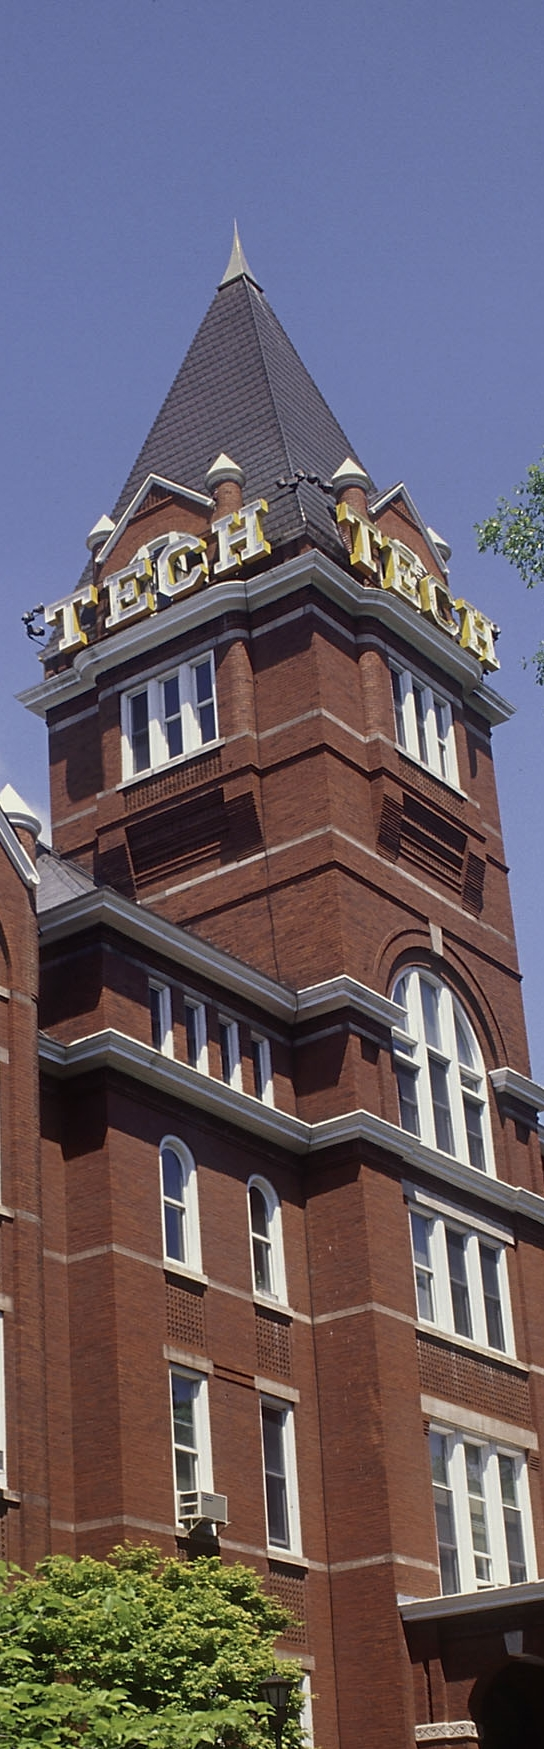
\includegraphics[width=1.25in]{figs/logo_TechTower.jpg}
    	\end{textblock}
    }

%logo tree
    \newcommand{\logoTree}
    {
    	\begin{textblock}{1}(0,0) 
    		\includegraphics[width=1.25in]{figs/logo_tree.jpg}
    	\end{textblock}
    }
%page numbers
    \newcommand{\mypagenum}
    {
    	\begin{textblock}{1}(1,94) 
		{\tiny \color[rgb]{0.2,0.2,1}\insertframenumber} %\insertframenumber,\insertpresentationendpage, \inserttotalframenumber
    	\end{textblock}
    }
%my footnote citation
	\newcommand{\myFootnoteCitation}[2]
	{
		\footnote{\tiny \citeauthor{#1}, \emph{#2}, \citeyear{#1}.}  %\citeauthor{#1}, \citetitle{#1}, #2 \citeyear{#1}.
	}
%my refer to citation
	\newcommand{\mycite}[1]
	{
		\emph{\citeauthor{#1} (\citeyear{#1})}
	}
%my footnote website citation
	\newcommand{\myFootnoteWebsiteCitation}[1]
	{
		\footnote{\tiny \citeauthor{#1}}
	}

\let\thefootnote\relax\footnotetext{Footnotetext without footnote mark}


%section underline
%\newcommand{\tmpsection}[1]{}
%\let\tmpsection=\section
%\renewcommand{\section}[1]{\tmpsection{\underline{#1}}}



%commands
	\newcommand{\likelihood}{p(Z_k| x_k) }						%likelihood
	\newcommand{\prior}{p(x_k)  } 								%prior
	\newcommand{\posterior} {p(x_k| Z_k)}						%posterior
	\newcommand{\prediction} {p(x_k| Z_{k-1})}					%prediction
	\newcommand{\update} {p(x_k|Z_k)}							%update
	\newcommand{\observations} {p(Z_k)}						%observations
	\newcommand{\prevobservations} {p(Z_{k-1})}				%previous observations
	\newcommand{\dxpk} {dx_{k-1}}							%dx_{k-1}
	\newcommand{\ChapKolm}{\int{p(x_k| x_{k-1})p(x_{k-1}|Z_{k-1})} \dxpk} %Chapman Kolmogorov

	%algorithm specific: JPDAF
	\newcommand{\likelihoodJPDAF}{p(Z_k| \chi, m, Z_{k-1}) }		%1. likelihood
	\newcommand{\priorJPDAF}{p(\chi|m, Z^{k-1}} 				%2. prior	
	\newcommand{\observationsJPDAF} {p(Z_k}					%3. observations
	\newcommand{\posteriorJPDAF} {p(\chi| Z_k)}					%4. posterior

%environments
	\newenvironment{changemargin}[2]
	{
	  	\begin{list}{}
		{
			\setlength{\topsep}{0pt}%
			\setlength{\leftmargin}{#1}%
			\setlength{\rightmargin}{#2}%
			\setlength{\listparindent}{\parindent}%
			\setlength{\itemindent}{\parindent}%
			\setlength{\parsep}{\parskip}%
		}
	  	\item[]
		}
		{\end{list}
	}
%figures

%colors
\definecolor{darkgreen}{rgb}{0,0.5,0}

%personal details
	\author{Salman Aslam}
	\institute{Advisor, Dr Christopher Barnes (ECE)\\Co-advisor, Dr Aaron Bobick (CoC)\\Georgia Institute of Technology}
	\date{}

\begin{document}
%####################################################################################################
\title{Target Tracking \\ Using \\Residual Vector Quantization}
%####################################################################################################
\begin{frame}[plain]\logoCSIPCPL\logoTechTower
	\titlepage
\end{frame}

\begin{frame}
\frametitle{Outline}
\logoCSIPCPL\logoTechTower
	\setcounter{tocdepth}{2}	
	\tableofcontents
\end{frame}

%####################################################################################################
\section{Background}
%####################################################################################################
\begin{frame}
\frametitle{Milestones}
\framesubtitle{}
\logoCSIPCPL\mypagenum
\vspace{0.2in}
\begin{itemize}
\item 2005: Dr Altunbasak, hierarchical motion vector estimation, background modeling
\item {\color{blue}Interest}: pattern recognition applied to images
\item 2007: switched to Dr Bobick, robust computer vision on compressed video
\item 2010: Dr Barnes + Dr Bobick, RVQ as a pattern recognition method extended to several images
\end{itemize}
\begin{figure}
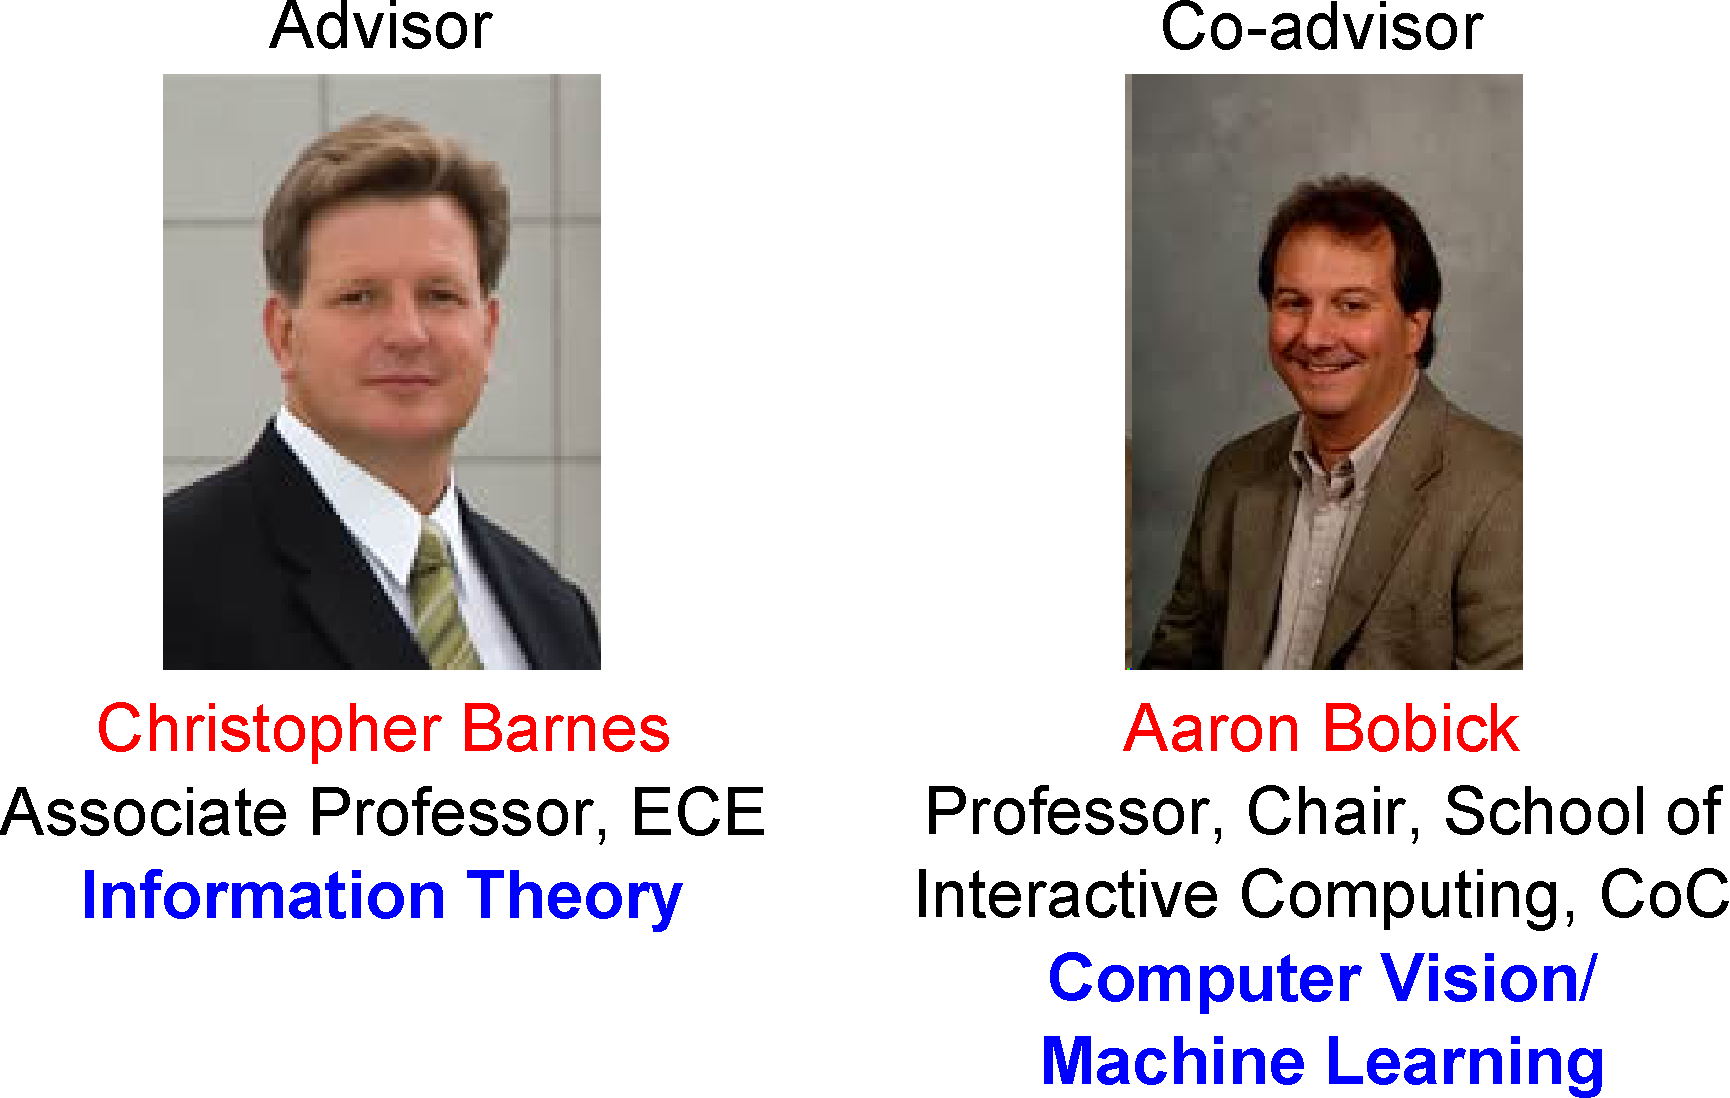
\includegraphics[width=0.8\textwidth]{thesis/professors.pdf}
\end{figure}
\end{frame}

%####################################################################################################
\section{Tracking}
%####################################################################################################
\begin{frame}
\frametitle{Tracking}
\framesubtitle{definition}
\logoCSIPCPL\mypagenum
	Estimate and maintain {\color{red}target state} over {\color{red}time}
	\begin{figure}
		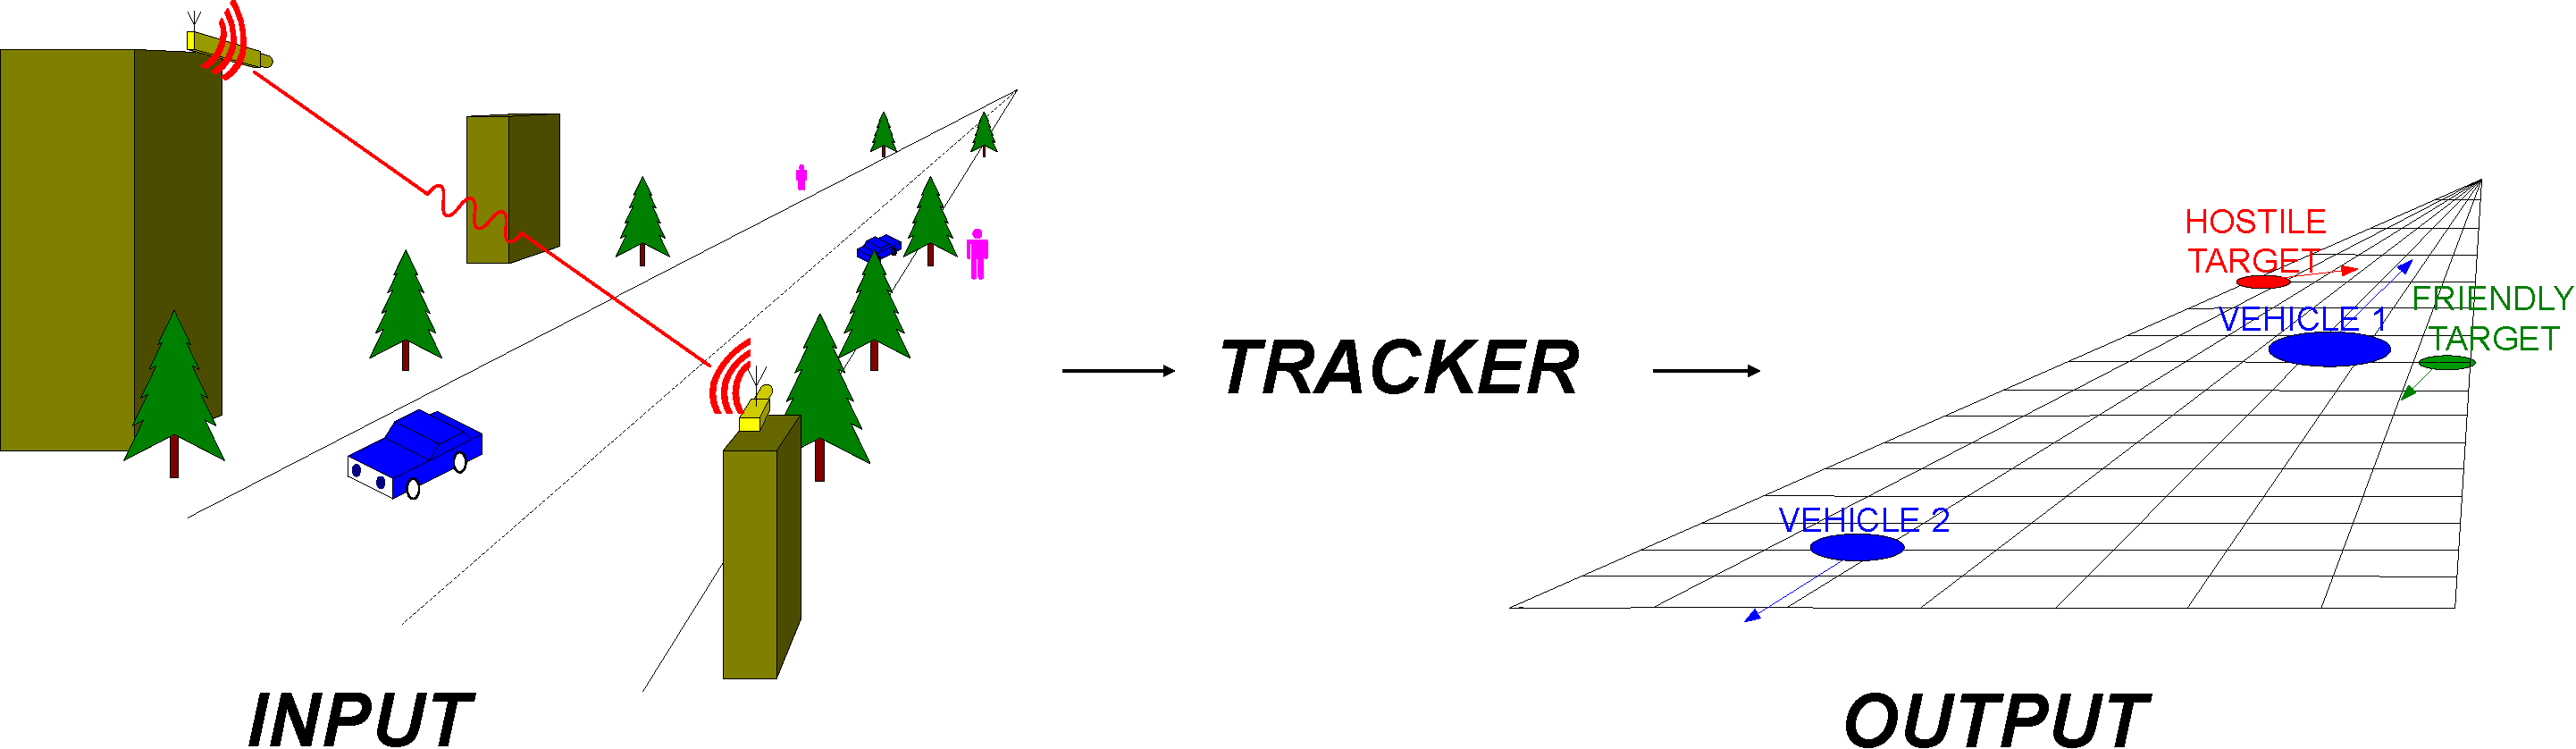
\includegraphics[width=1.0\textwidth]{thesis/TRK_overviewDiagram.pdf}
	\end{figure}
\end{frame}


\begin{frame}[plain]
\frametitle{Tracking}
\framesubtitle{overview\tiny{\footnote {Yilmaz et.al., 2006}}}
\logoCSIPCPL\mypagenum
	\begin{changemargin}{-1.3in}{0in}
		\begin{figure}
			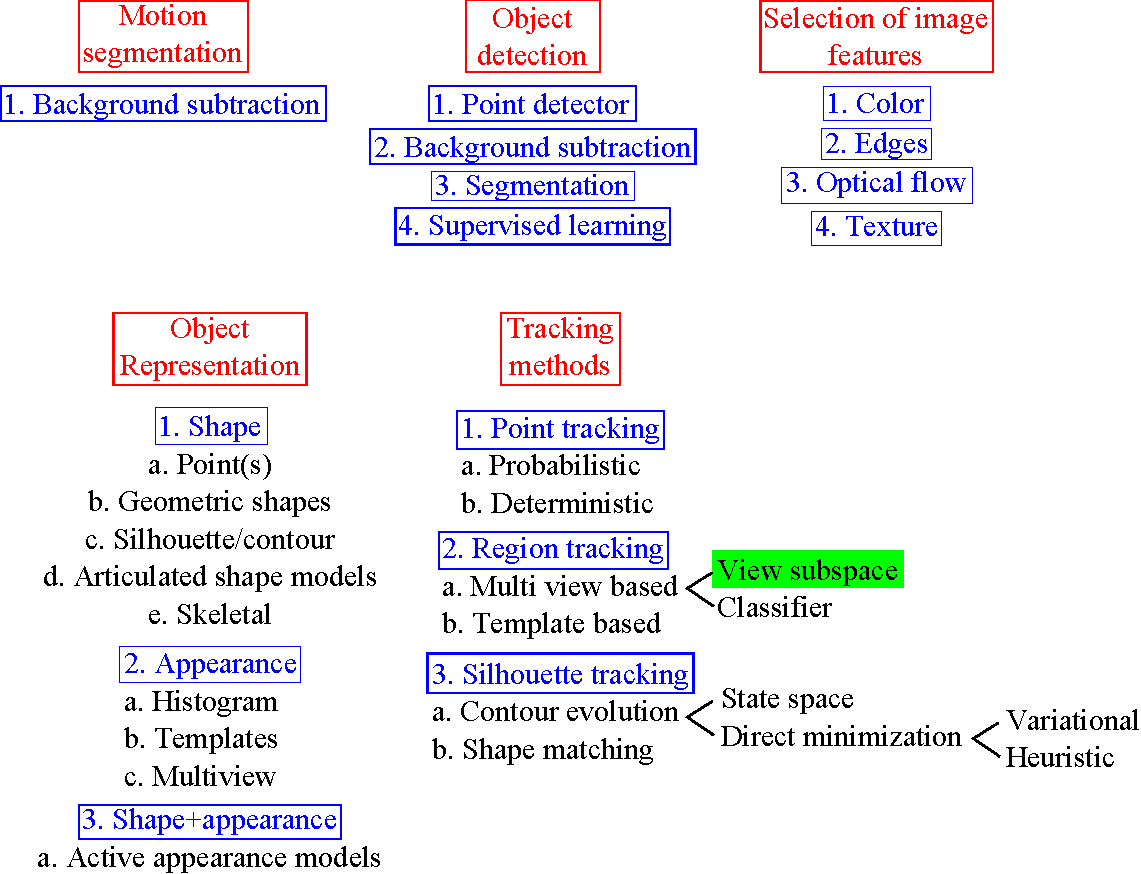
\includegraphics[width=1.3\textwidth]{thesis/TRK_overview.pdf}
		\end{figure}	
	\end{changemargin}
	\begin{block}{Tracking methods}
		\begin{itemize}
			\item Point
			\item Region
			\item Contour
		\end{itemize}
	\end{block}
\end{frame}



\begin{frame}
\frametitle{Tracking}
\framesubtitle{big picture}
\logoCSIPCPL\mypagenum
	\begin{figure}
		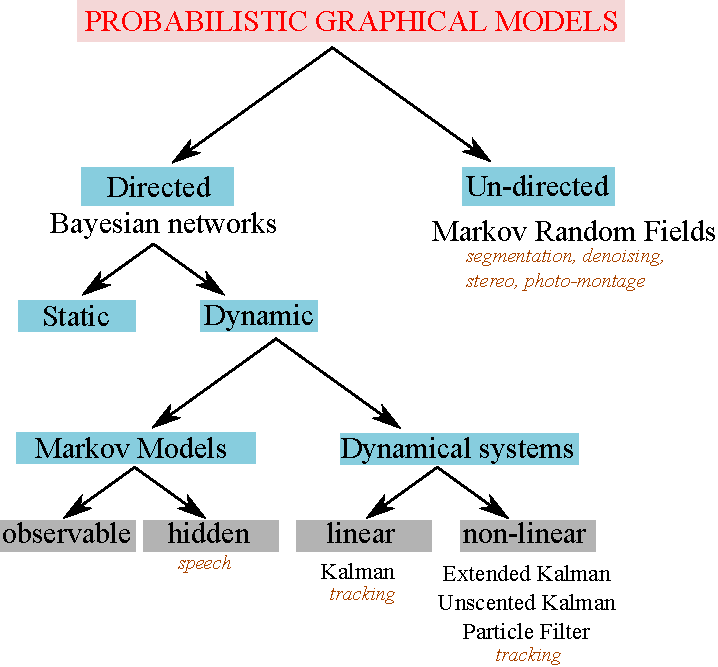
\includegraphics[width=0.9\textwidth]{thesis/PRML_PGM_overview.pdf}
	\end{figure}
\end{frame}





\begin{frame}
\frametitle{Tracking}
\framesubtitle{relationship with HMM}
\logoCSIPCPL\mypagenum
	\begin{figure}
		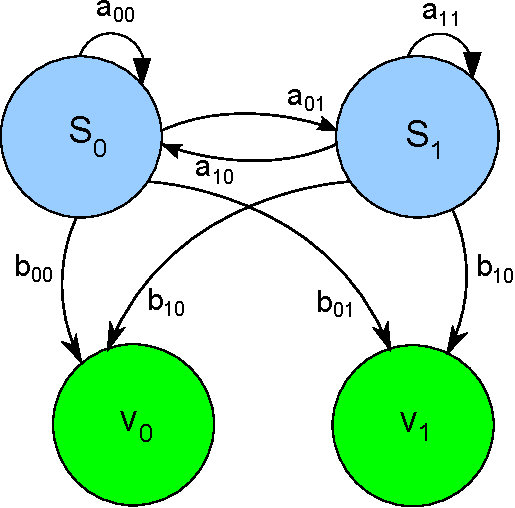
\includegraphics[height=0.3\textheight]{thesis/HMM_flowDiagram.pdf}
	\end{figure}
	\begin{figure}
		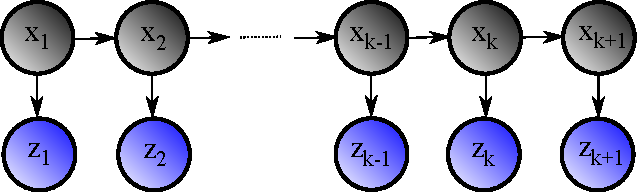
\includegraphics[width=1.0\textwidth]{thesis/HMM_flowDiagram2.pdf}
	\end{figure}
\end{frame}



\begin{frame}
\frametitle{Tracking}
\framesubtitle{update}
\logoCSIPCPL\mypagenum
	\begin{figure}
		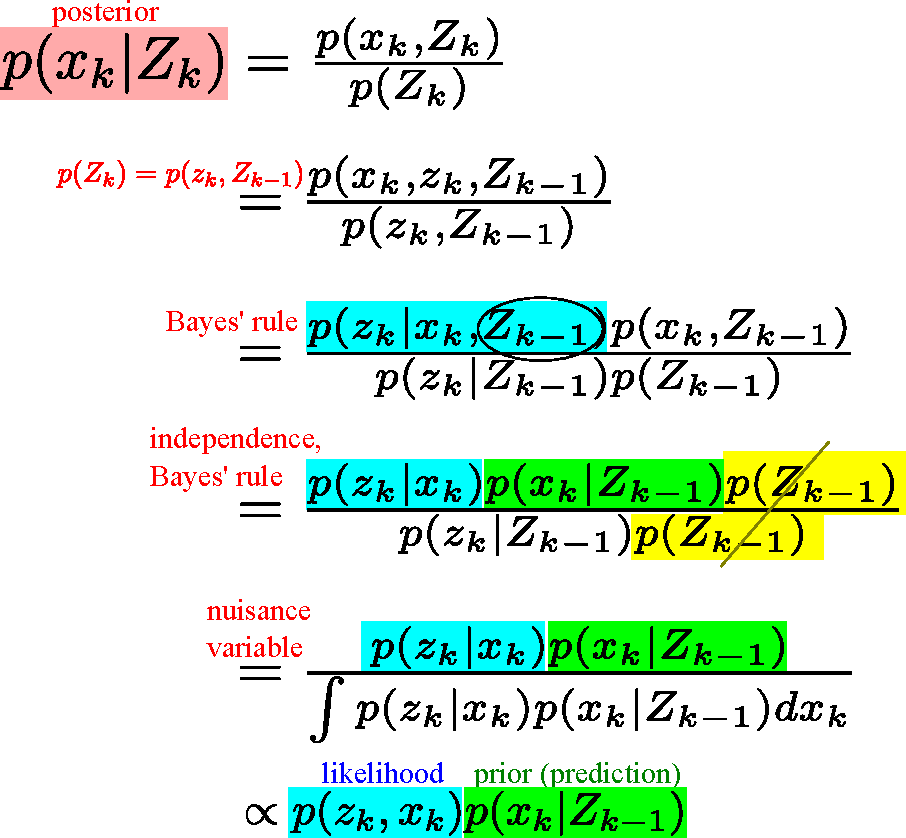
\includegraphics[width=1.0\textwidth]{thesis/TRK_EQN_update.pdf}
	\end{figure}
\end{frame}



\begin{frame}
\frametitle{Tracking}
\framesubtitle{prediction}
\logoCSIPCPL\mypagenum
	Chapman Kolmogorov equation
	\begin{figure}
		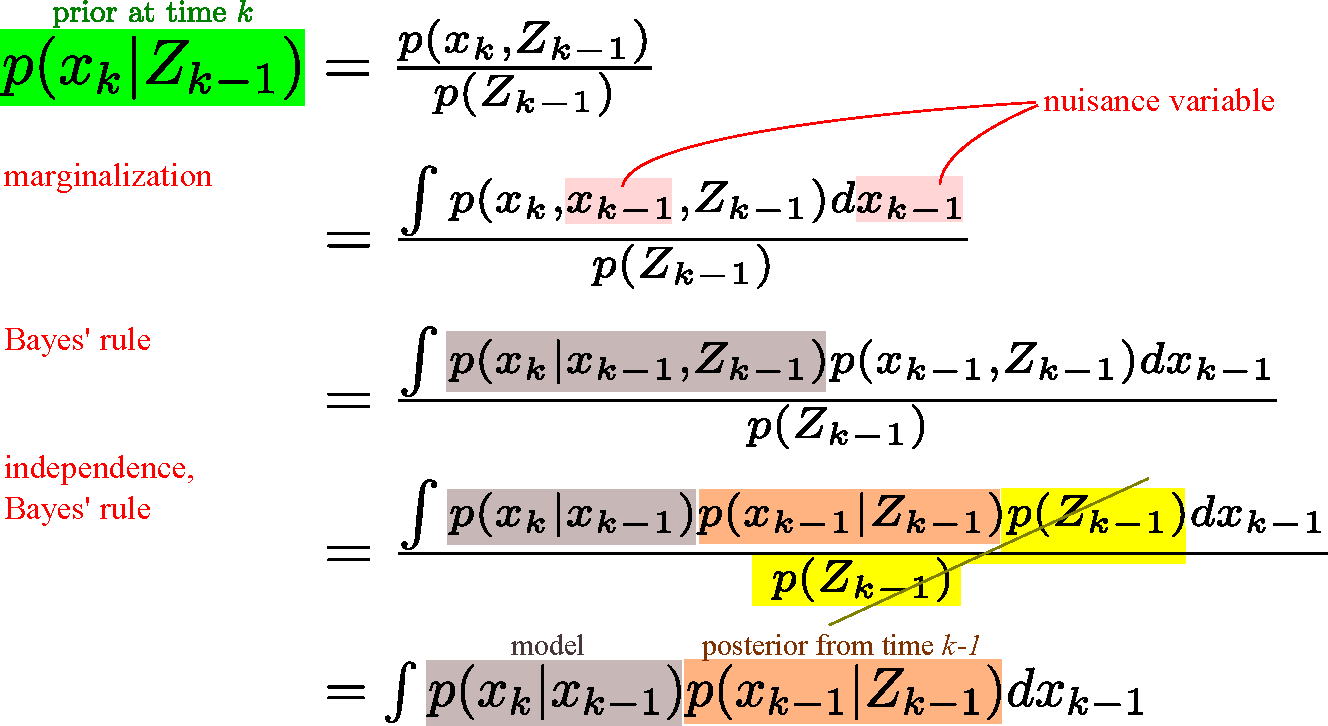
\includegraphics[width=1.0\textwidth]{thesis/TRK_EQN_prediction.pdf}
	\end{figure}
\end{frame}


\begin{frame}
\frametitle{Origin: radar}
\framesubtitle{Kalman Filter}
\logoCSIPCPL\mypagenum
	\begin{figure}
		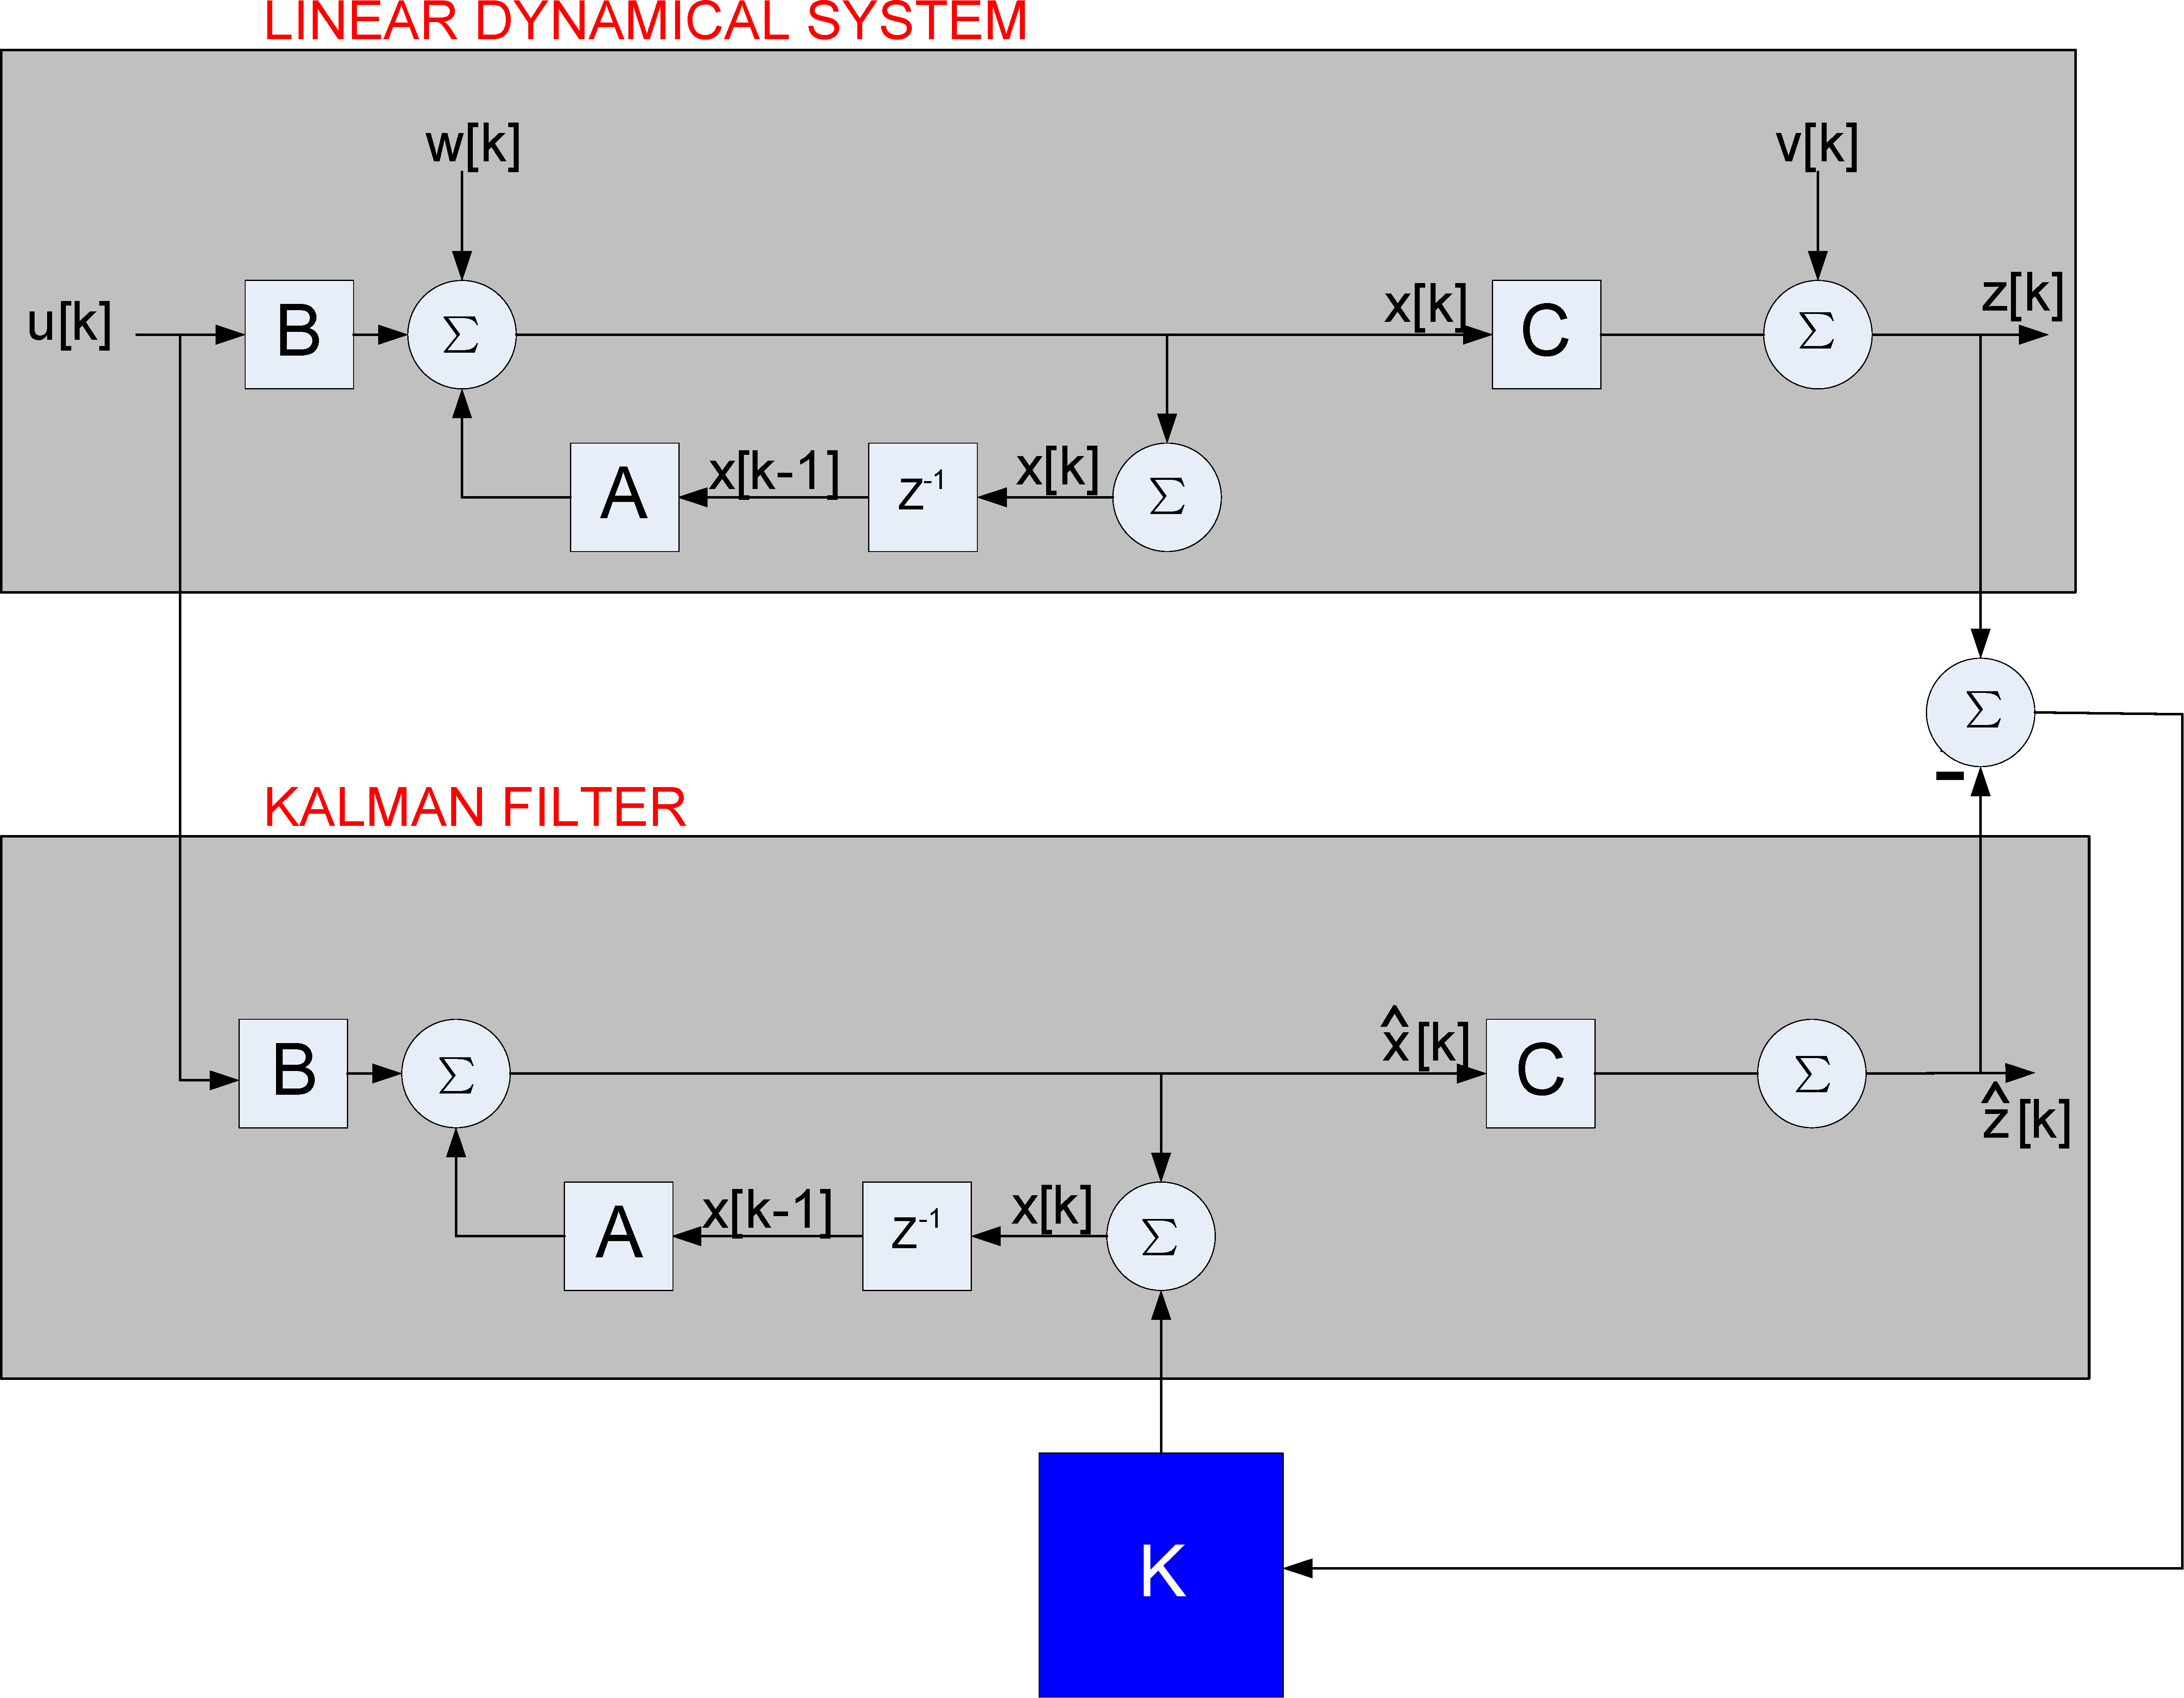
\includegraphics[width=1.0\textwidth]{thesis/TRK_KalmanFilter_blockDiagram.pdf}
	\end{figure}
\end{frame}

\begin{frame}
\frametitle{Particle Filter}
\framesubtitle{multi-modal PDF}
\logoCSIPCPL\mypagenum
	\begin{figure}
		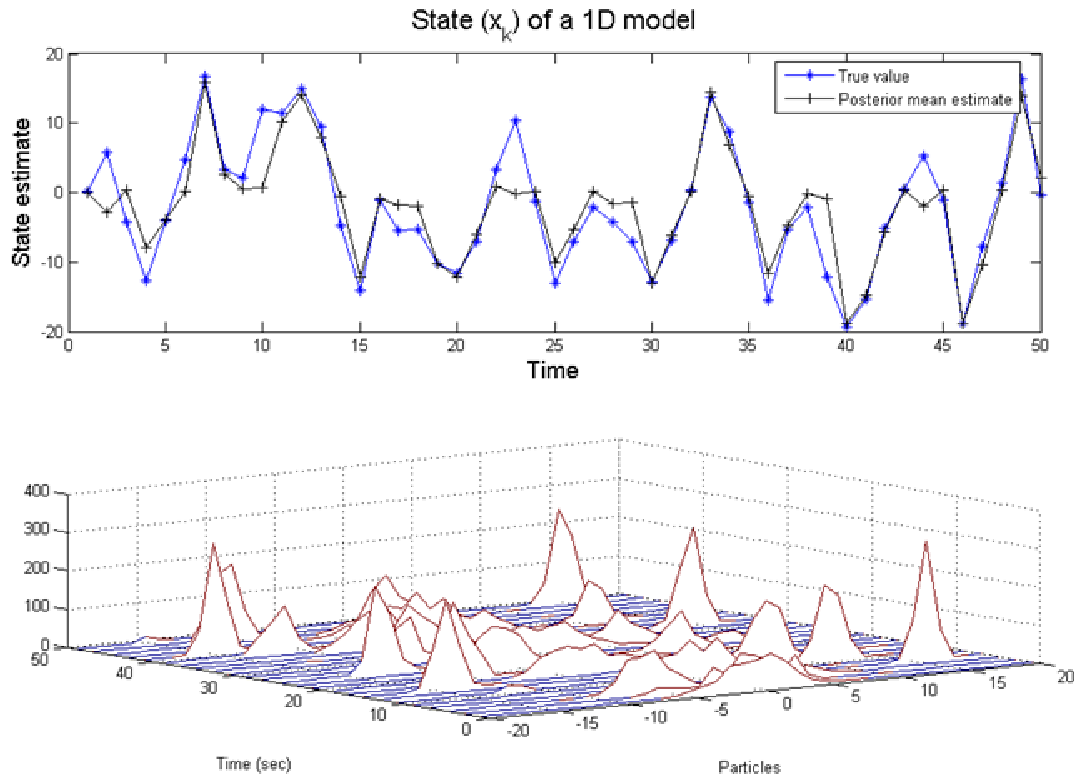
\includegraphics[width=1.0\textwidth]{thesis/TRK_ParticleFilter_multimodalPDF.pdf}
	\end{figure}	
\end{frame}


\begin{frame}
\frametitle{Pre-processing}
\logoCSIPCPL\mypagenum
	{\color{red}Steps}
	\begin{enumerate}
		\item Downsampling
		\item Normalization
		\item Stabilization
		\item Background modeling
		\item Feature Extraction
	\end{enumerate}
	\vspace{0.3in}
	{\color{red}Features}
	\begin{enumerate}
		\item Color
		\item Edges
		\item Corners
		\item Motion
		\item Texture
		\item Depth
		\item Density
	\end{enumerate}
\end{frame}









%===================================================
\subsection{\ \ \ \ region}
%===================================================
\begin{frame}
\frametitle{Region tracking}
\framesubtitle{overview}
\logoCSIPCPL\mypagenum
	\begin{enumerate}
		\item Template matching
			\begin{itemize}
				\item fixed templates: reliable over short durations 
			\end{itemize}
		\item Subspace methods
			\begin{itemize}
				\item usually learned with PCA
				\item model variations in lighting and pose
				\item disadvantages: object specific, training
			\end{itemize}			
		\item Probability density
			\begin{itemize}
				\item robustness under image distortions and occlusions
				\item fast to learn
				\item disadvantage: lack of expressiveness, registration can be difficult
			\end{itemize}
		\item Motion
			\begin{itemize}
				\item optical flow works well for small displacements
				\item block matching for large motion
				\item computing motion vectors is computationally complex
			\end{itemize}
	\end{enumerate}
\end{frame}


%####################################################################################################
\section{RVQ}
%####################################################################################################
%===================================================
\subsection{\ \ \ \ introduction}
%===================================================

\begin{frame}
\frametitle{Quantization}
\framesubtitle{overview}
\logoCSIPCPL\mypagenum
	\begin{figure}				
		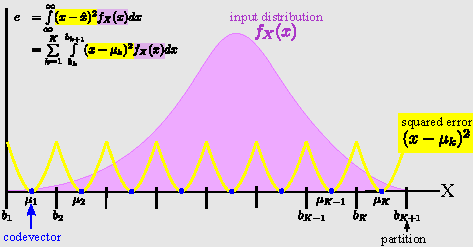
\includegraphics[width=0.9\textwidth]{thesis/Quantization_MSE.pdf}
	\end{figure}
\end{frame}





\begin{frame}[plain]
\frametitle{Lloyd Max conditions}
\framesubtitle{Optimal code-vectors}
\logoCSIPCPL\mypagenum
	\begin{changemargin}{-1.3in}{0in}
		\begin{figure}				
			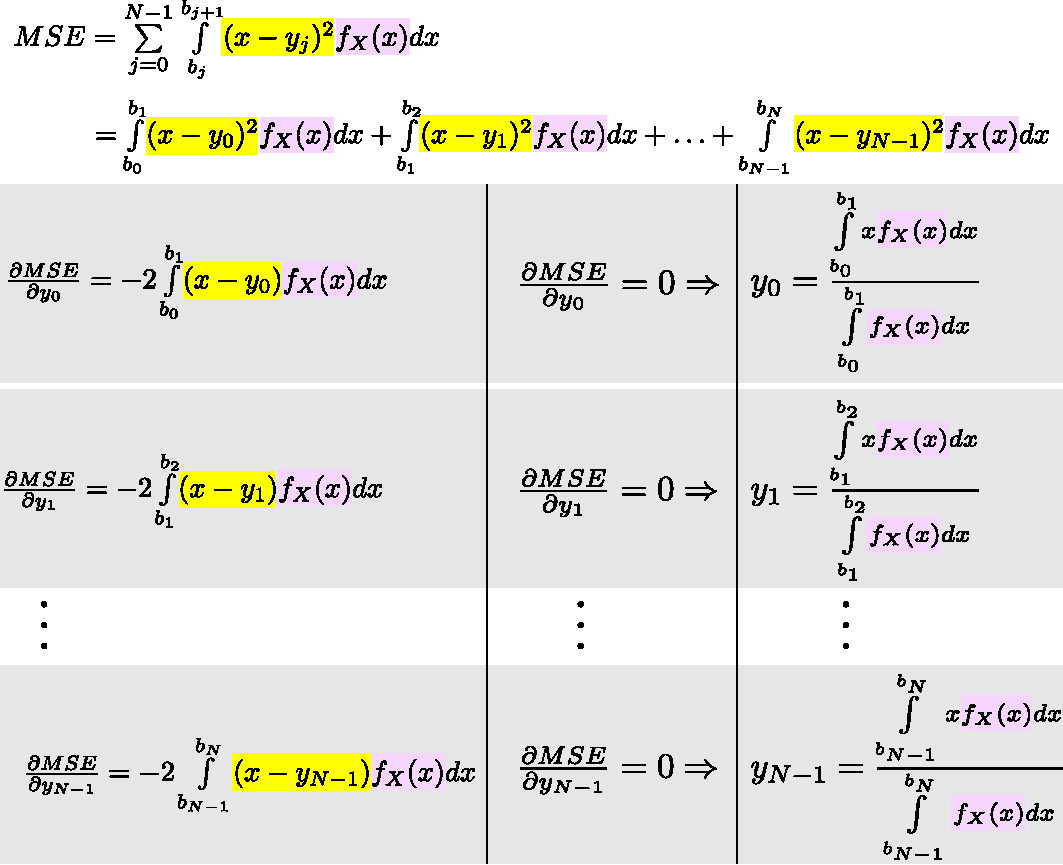
\includegraphics[height=0.8\textheight]{thesis/Quantization_optimalCodevectors.pdf}
		\end{figure}
	\end{changemargin}
\end{frame}



\begin{frame}
\frametitle{Lloyd Max conditions}
\framesubtitle{Optimal partitions}
\logoCSIPCPL\mypagenum
	\begin{figure}				
		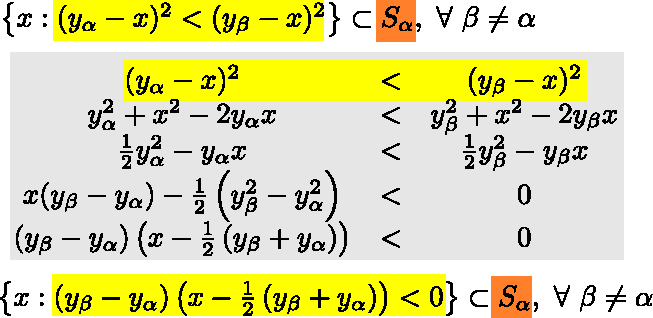
\includegraphics[width=1.0\textwidth]{thesis/Quantization_optimalPartitions.pdf}
	\end{figure}
\end{frame}



\begin{frame}[plain]
\frametitle{Lloyd Max conditions}
\framesubtitle{Optimal partitions (cont.)}
\logoCSIPCPL\mypagenum
	\begin{changemargin}{-1.3in}{0in}
		\begin{figure}				
			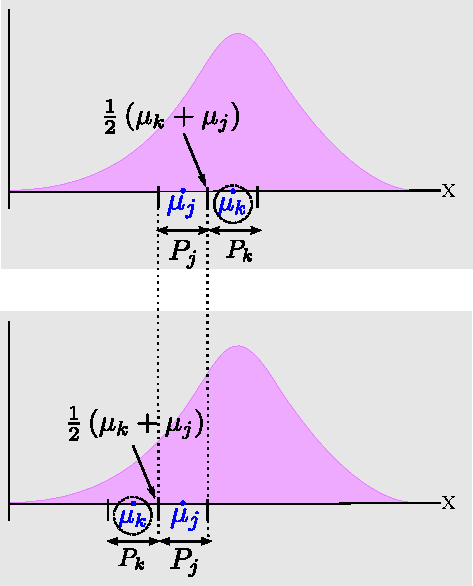
\includegraphics[height=0.8\textheight]{thesis/Quantization_optimalPartitions2.pdf}
		\end{figure}
	\end{changemargin}
\end{frame}


\begin{frame}
\frametitle{Vector Quantization}
\framesubtitle{types}
\logoCSIPCPL\mypagenum
	\begin{itemize}
		\item Unstructured
			\begin{itemize}
				\item Exhaustive Search (ESVQ)
			\end{itemize}
		\item Structured
		\begin{itemize}
			\item Tree Structured (TSVQ)
			\item Transform
			\item Product
				\begin{itemize}
					\item Mean-removed
					\item Shape-gain
					\item Residual (RVQ)
				\end{itemize}
		\end{itemize}
	\end{itemize}
\end{frame}




\begin{frame}[plain]
\frametitle{RVQ}
\framesubtitle{block diagram}
\logoCSIPCPL\mypagenum
	\begin{changemargin}{-1.3in}{0in}
		\begin{figure}				
			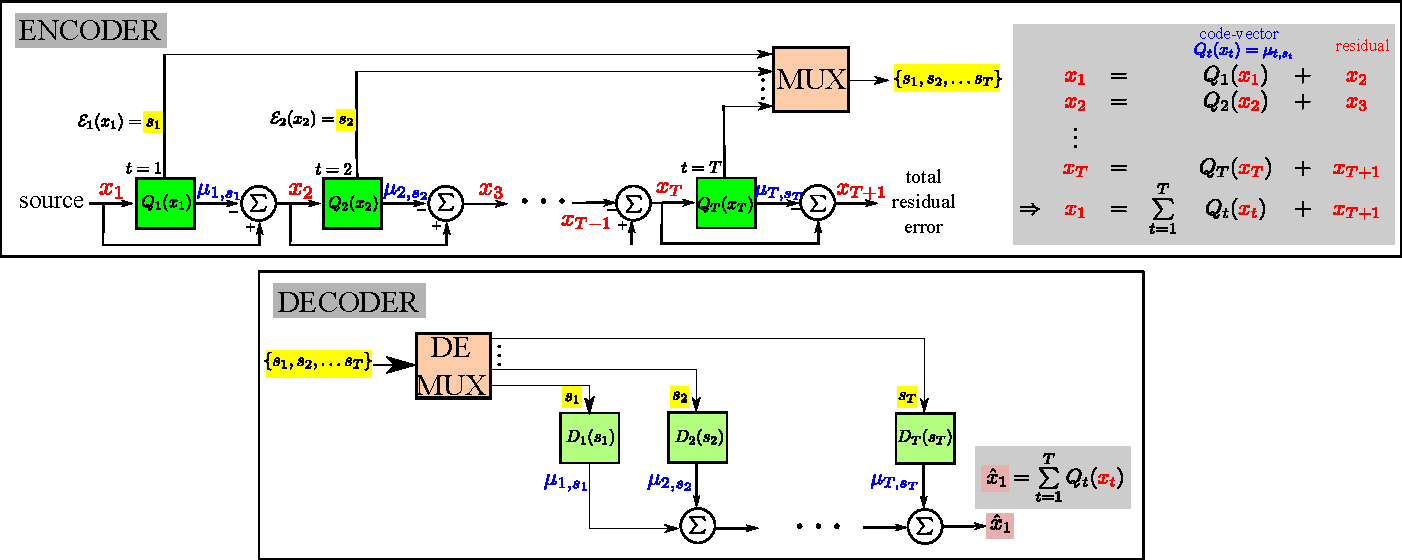
\includegraphics[width=1.3\textwidth]{thesis/RVQ_blockDiagram.pdf}
		\end{figure}
	\end{changemargin}
\end{frame}


%\begin{frame}
%\frametitle{RVQ}
%\framesubtitle{distortion}
%\logoCSIPCPL\mypagenum
%	\begin{figure}				
%		\includegraphics[width=1.0\textwidth]{thesis/RVQ_distortion.pdf}
%	\end{figure}
%\end{frame}



\begin{frame}
\frametitle{RVQ}
\framesubtitle{tree structure}
\logoCSIPCPL\mypagenum
	\begin{figure}				
		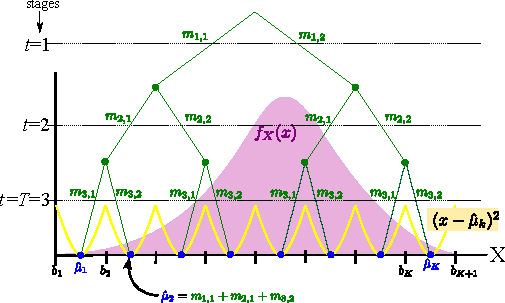
\includegraphics[width=1.0\textwidth]{thesis/RVQ_graphicalReconstruction.pdf}
	\end{figure}
\end{frame}




\begin{frame}[plain]
\frametitle{RVQ}
\framesubtitle{derivation}
\logoCSIPCPL\mypagenum
	\begin{changemargin}{-1.3in}{0in}
		\begin{figure}				
			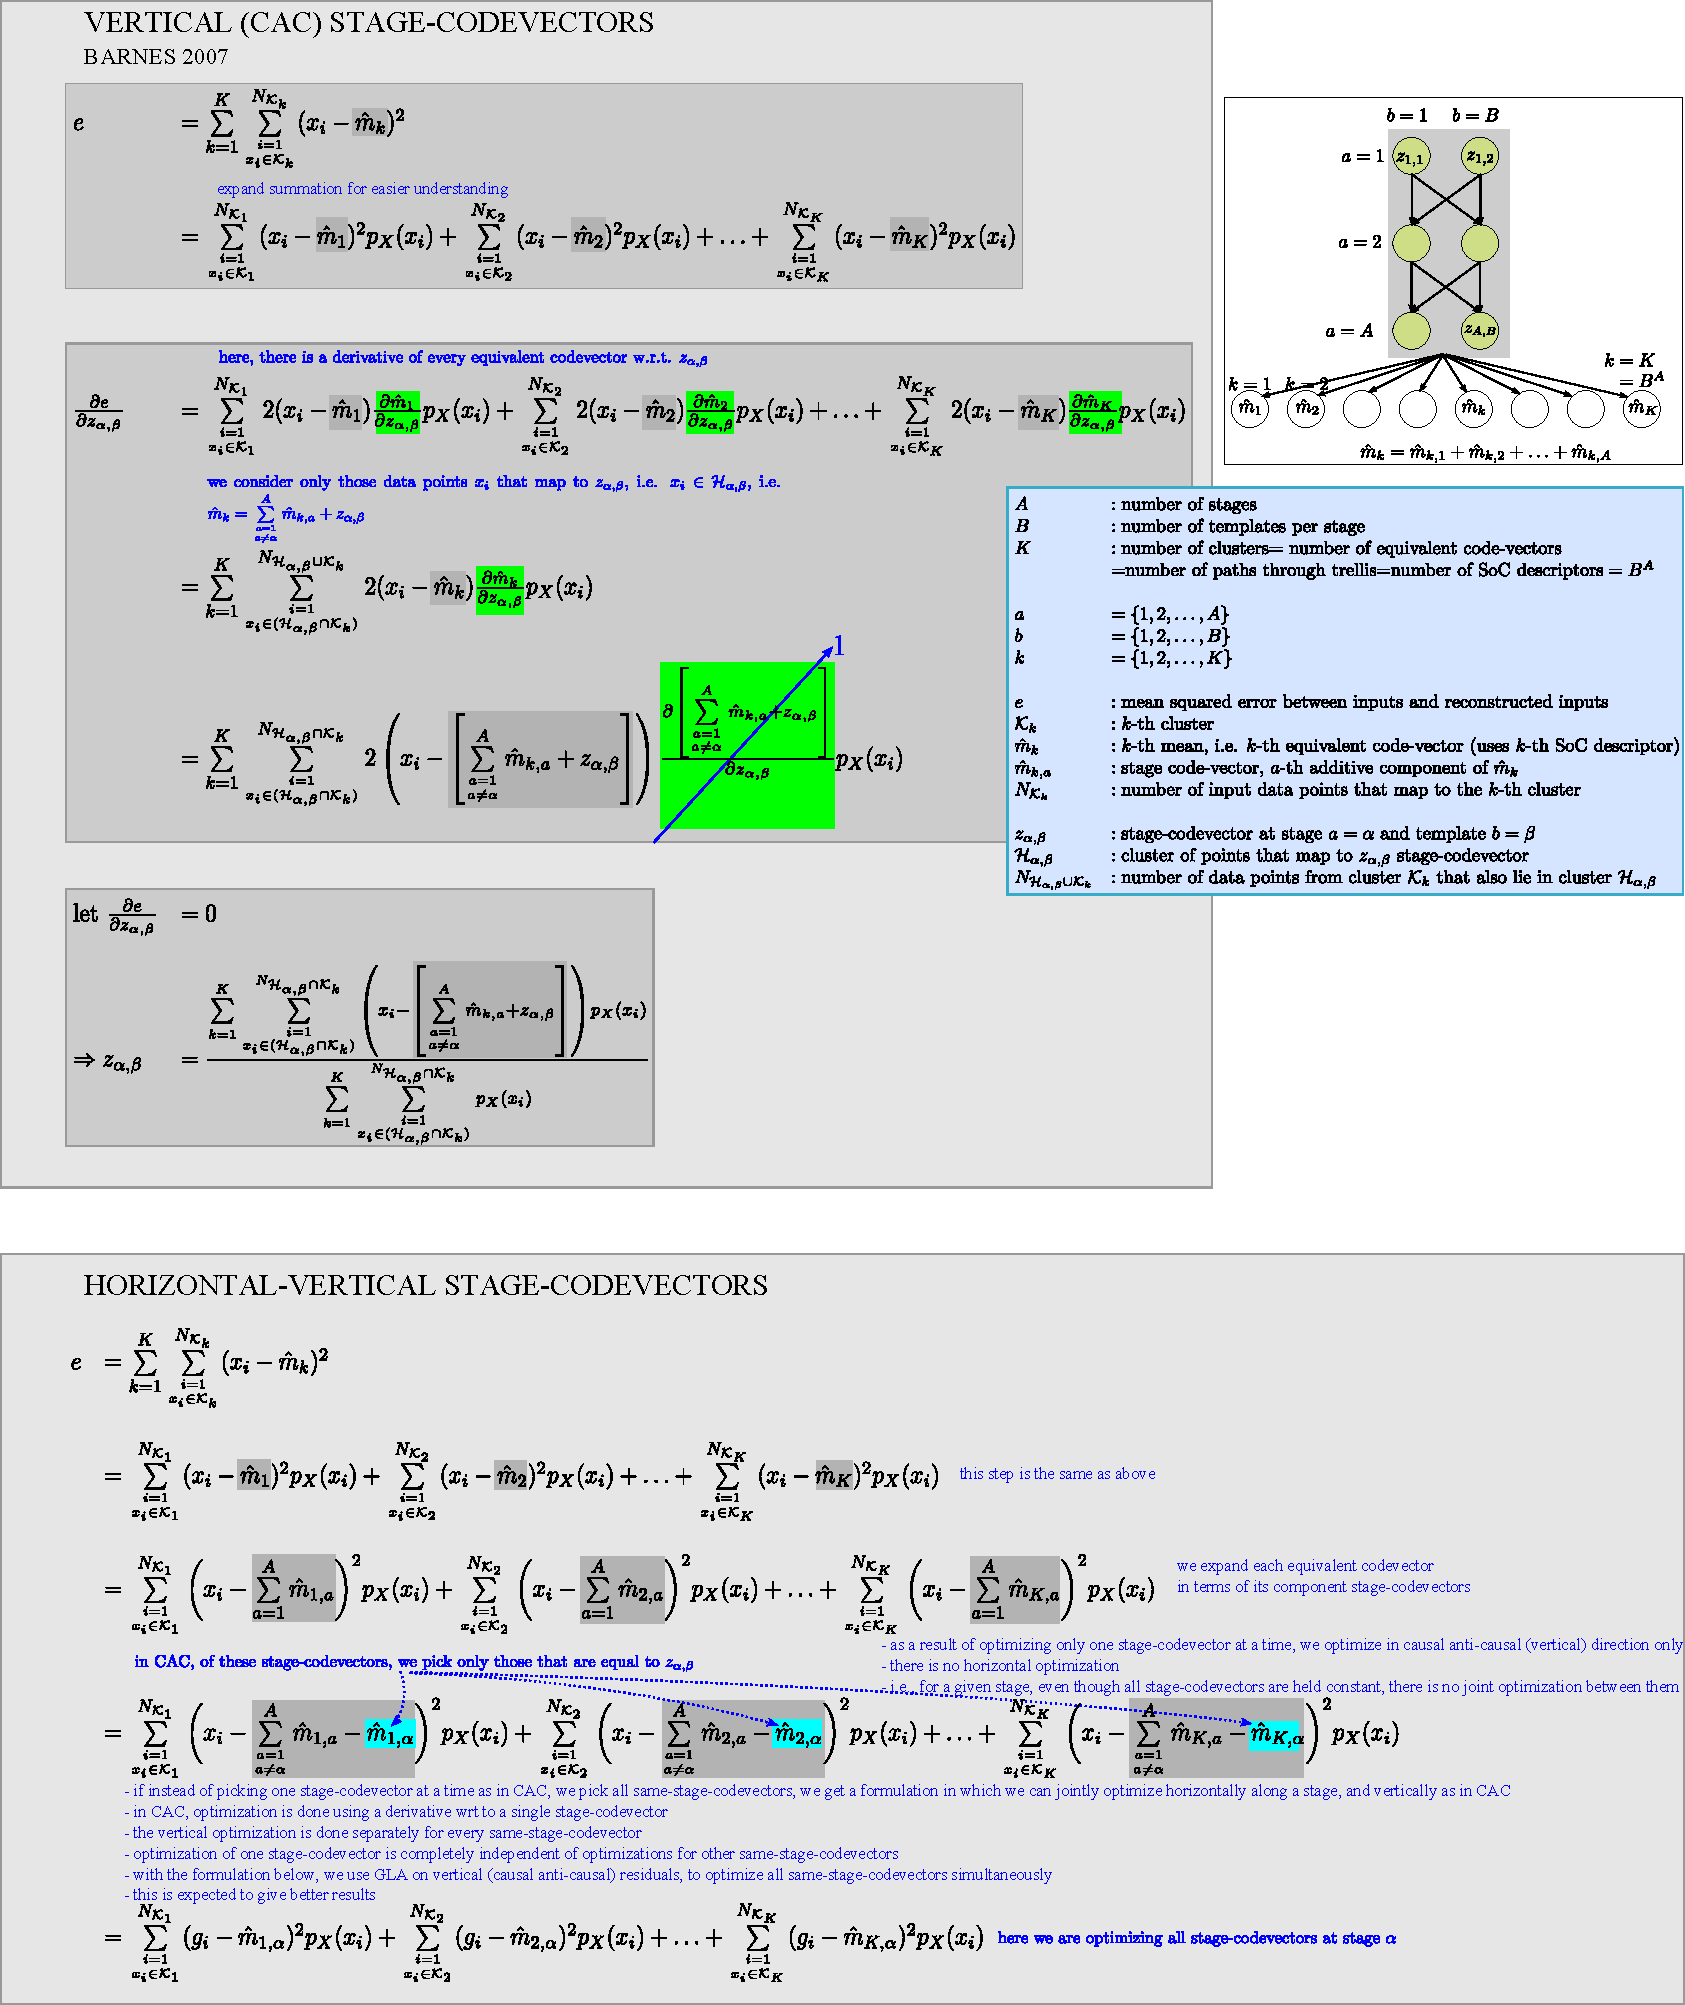
\includegraphics[width=1.3\textwidth]{thesis/RVQ_CAC_derivation.pdf}
		\end{figure}
	\end{changemargin}
\end{frame}


%===================================================
\subsection{\ \ \ \ comparisons}
%===================================================
\begin{frame}
\frametitle{RVQ comparison}\logoCSIPCPL\mypagenum
\framesubtitle{1. with ESVQ}
	\begin{itemize}
		\item ESVQ
			\begin{itemize}
				\item $N=2^{rk}$ code-vectors
				\item Computations: $O(2^{rk})$
				\item Memory: $O(2^{rk})$
				\item Exponential in computations and memory
			\end{itemize}
		\item RVQ
			\begin{itemize}
				\item $N={M^P}$ code-vectors
				\item M code-vectors for each of P stages
				\item Computations: $O(MP)$
				\item Memory: $O(MP)$
				\item Linear in computations and memory
			\end{itemize}
	\end{itemize}
	Generally, structurally constrained quantizers cannot provide performance as good as ESVQ
	\begin{itemize}
		\item RVQ can handle higher dimensions due to linear complexity
		\item Better performance than ESVQ possible, for given implementation cost
	\end{itemize}	
\end{frame}


\begin{frame}[plain]
\frametitle{RVQ comparison}
\framesubtitle{2. with TSVQ}
\logoCSIPCPL\mypagenum
%	\begin{changemargin}{-1.3in}{0in}
%		\begin{figure}				
%			\includegraphics[width=1.3\textwidth]{thesis/RVQ_comparisonWithTSVQ.pdf}
%		\end{figure}
%	\end{changemargin}
\end{frame}



%\begin{frame}[plain]
%\frametitle{RVQ comparison}
%\framesubtitle{3. with PCA}
%\logoCSIPCPL\mypagenum
%	\begin{changemargin}{-1.3in}{0in}
%		\begin{figure}				
%			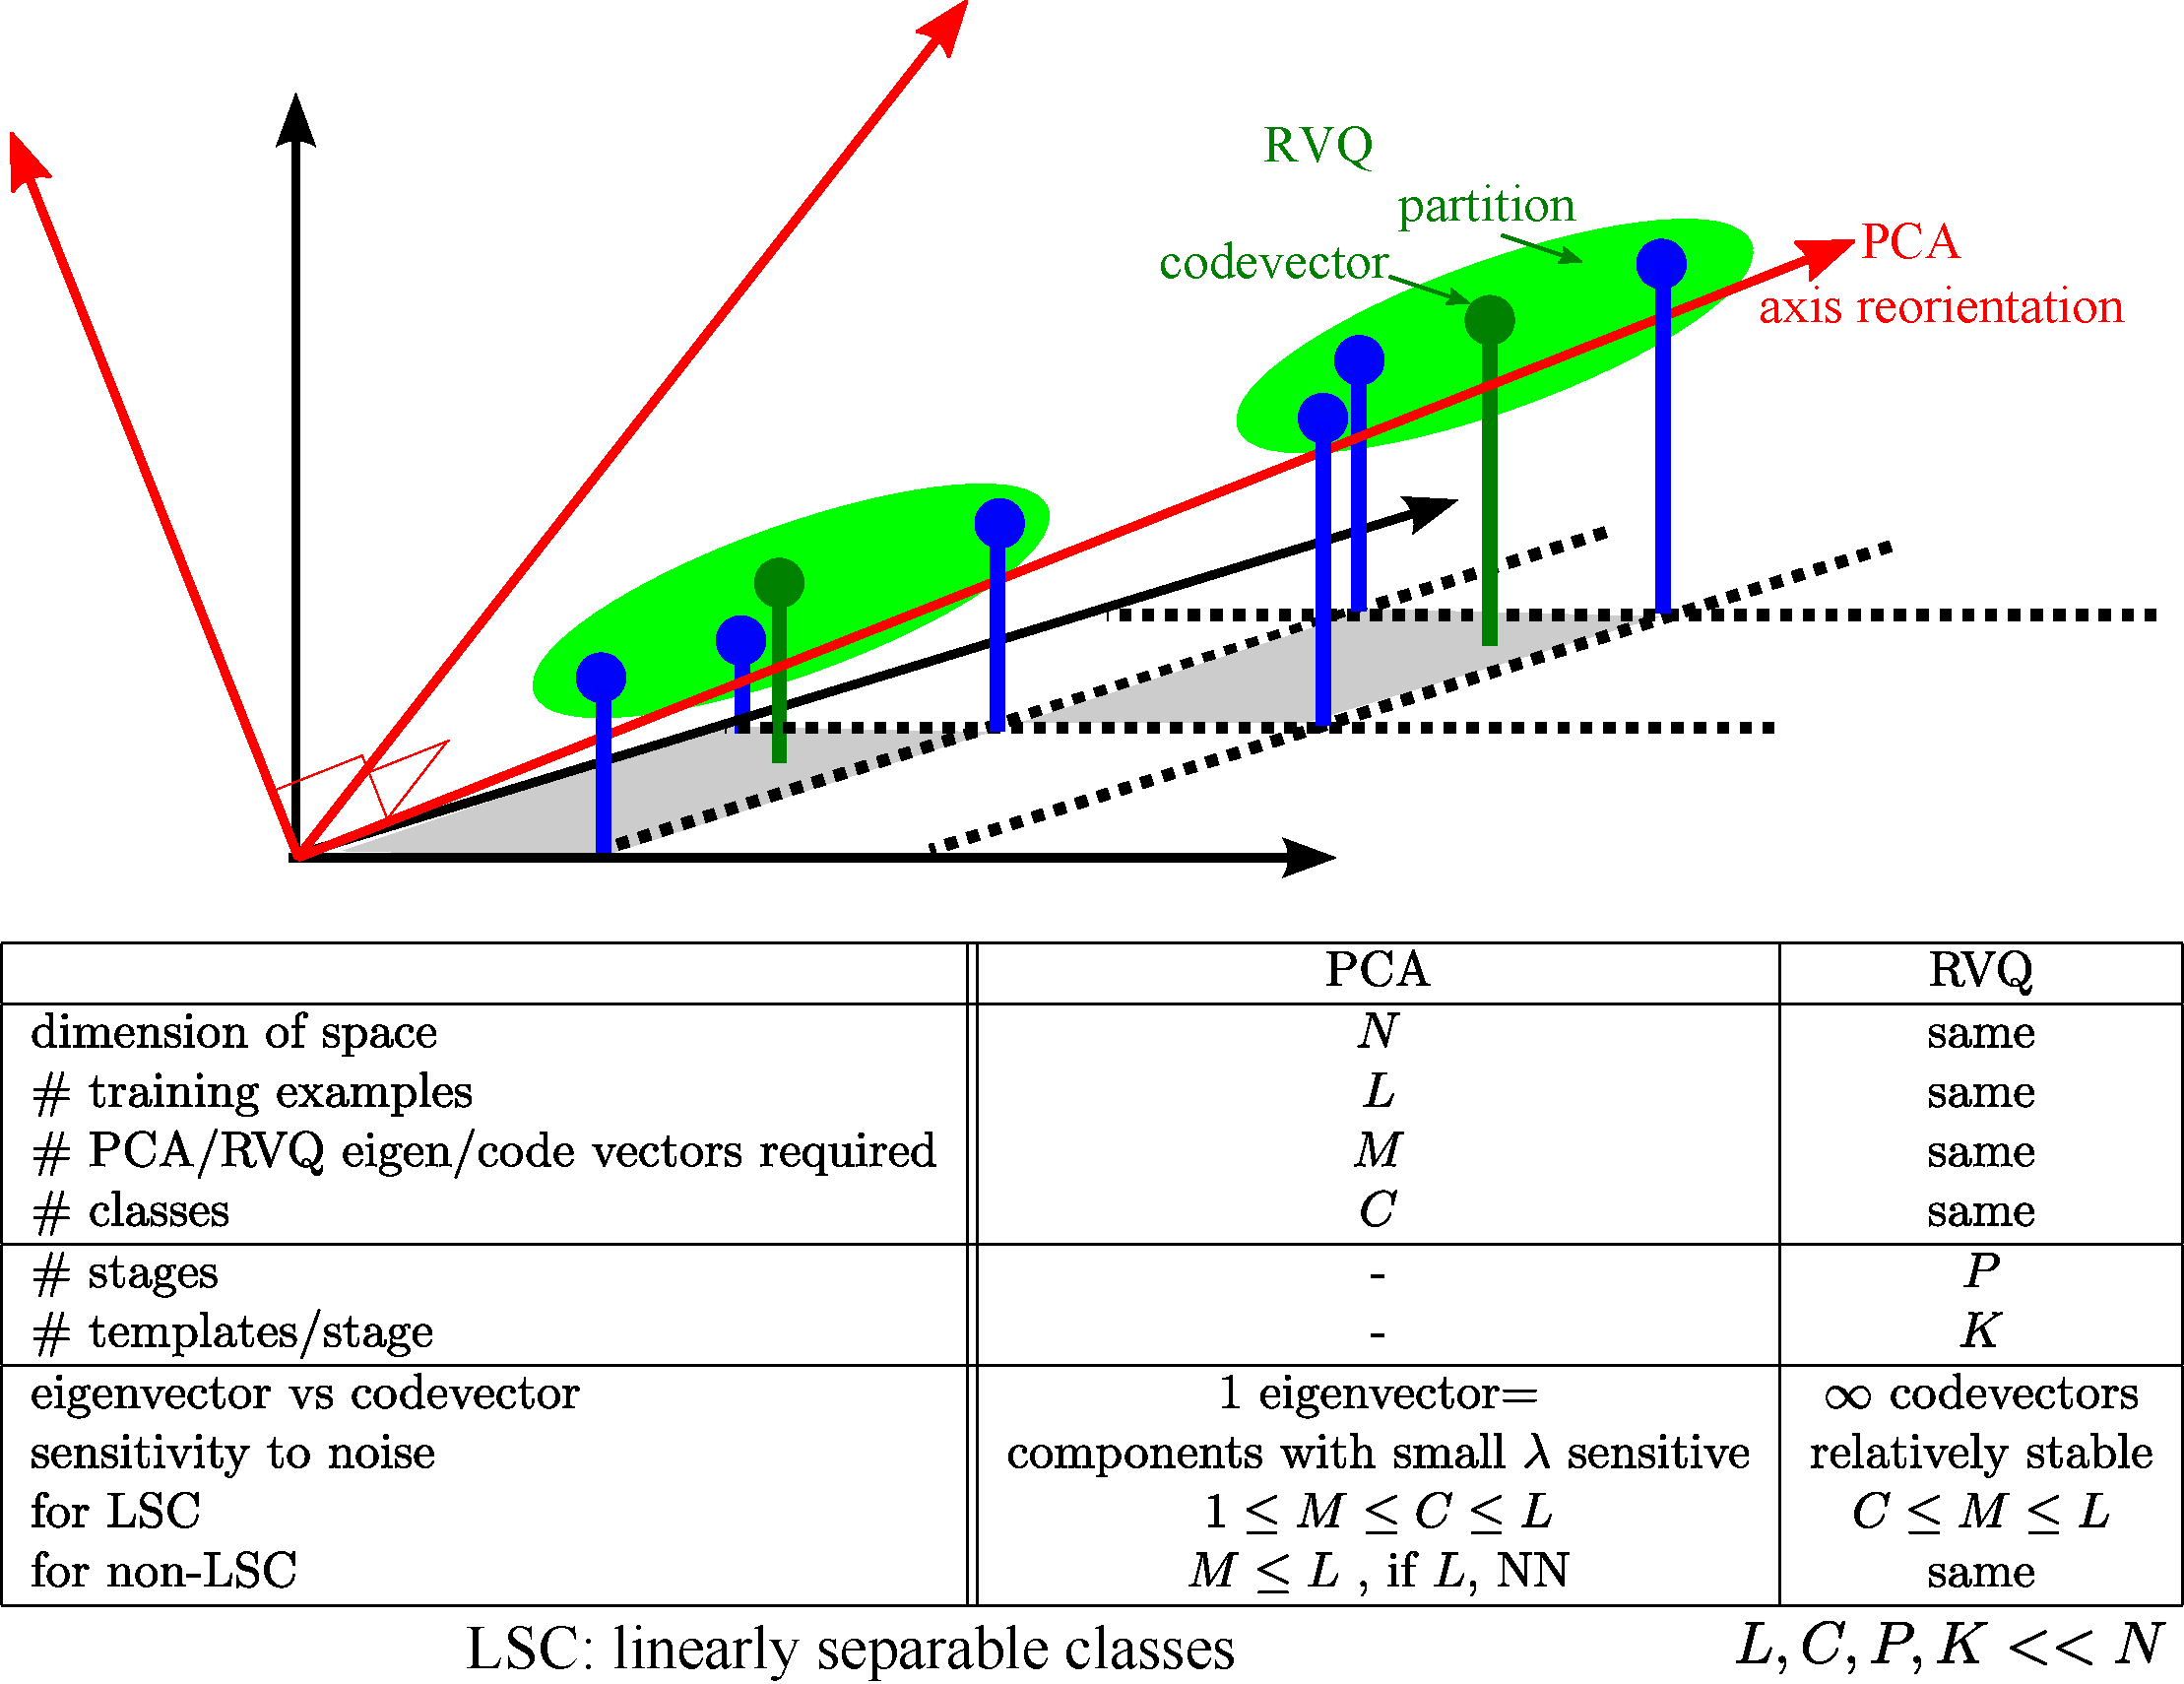
\includegraphics[width=1.3\textwidth]{thesis/RVQ_comparisonWithPCA.pdf}
%		\end{figure}
%	\end{changemargin}
%\end{frame}


%--------------------------------------------------------
\subsection{\ \ \ \ usage: image analysis}
%--------------------------------------------------------




\begin{frame}
\frametitle{RVQ classification}
\framesubtitle{\small Satellite imagery: pre-Tsunami Sri Lanka \\(training phase)}
\logoCSIPCPL\mypagenum
	\begin{figure}		
		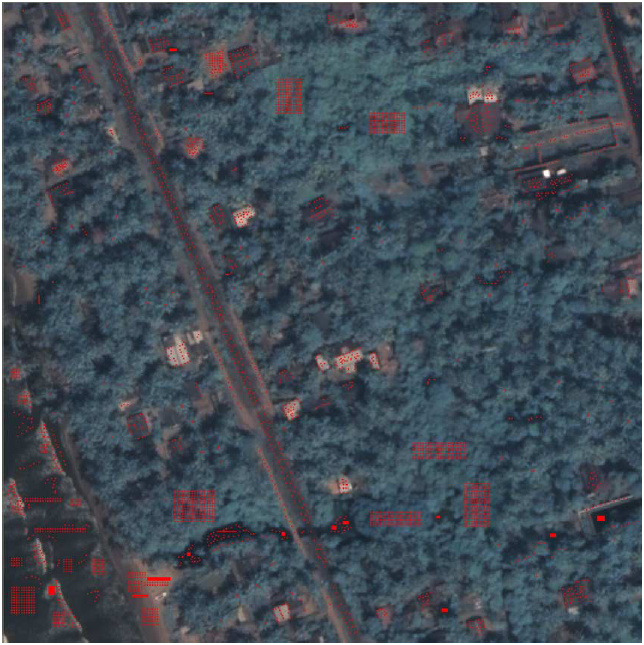
\includegraphics[height=0.35\textheight]{thesis/RVQ_SatelliteSriLanka_1_snippets.png}			
	\end{figure}
	\begin{figure}		
		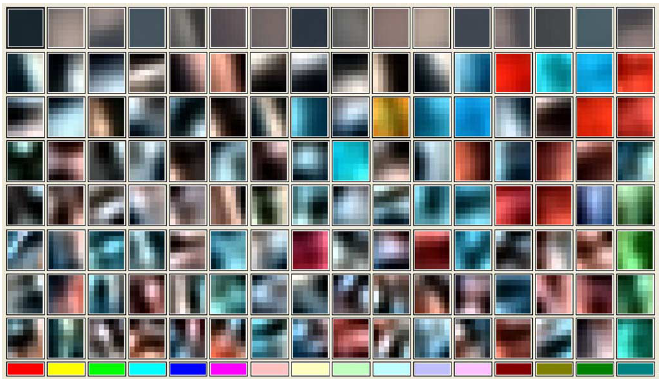
\includegraphics[height=0.40\textheight]{thesis/RVQ_SatelliteSriLanka_2_codebooks.png}			
	\end{figure}
\end{frame}




\begin{frame}
\frametitle{RVQ classification}
\framesubtitle{\small Satellite imagery: pre-Tsunami Sri Lanka\\(testing phase)}
\logoCSIPCPL\mypagenum
	\begin{figure}		
		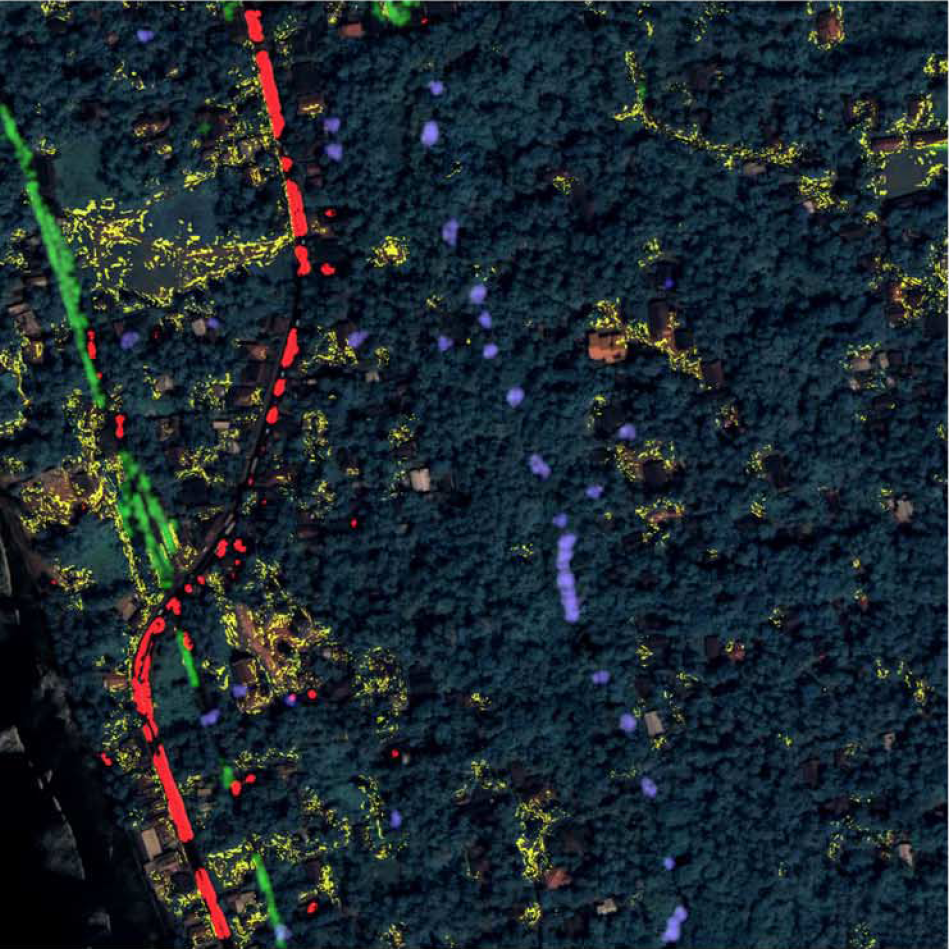
\includegraphics[height=0.6\textheight]{thesis/RVQ_SatelliteSriLanka_3_labeling.png}
		\caption{\hspace{1.3in}{\color{yellow}yellow}: dirt paths \\\hspace{1.3in}{\color{blue}blue}: rivers \\\hspace{1.3in}{\color{red}red}: paved roads \\\hspace{1.3in}{\color{green}green}: train tracks}
	\end{figure}
\end{frame}


%####################################################################################################
\section{RVQ tracking}
%####################################################################################################

\begin{frame}
\frametitle{RVQ classification}
\framesubtitle{$\mathbb{R}^{1089}$}
\logoCSIPCPL\mypagenum
\begin{figure}[t]
\subfigure[Uniform.]{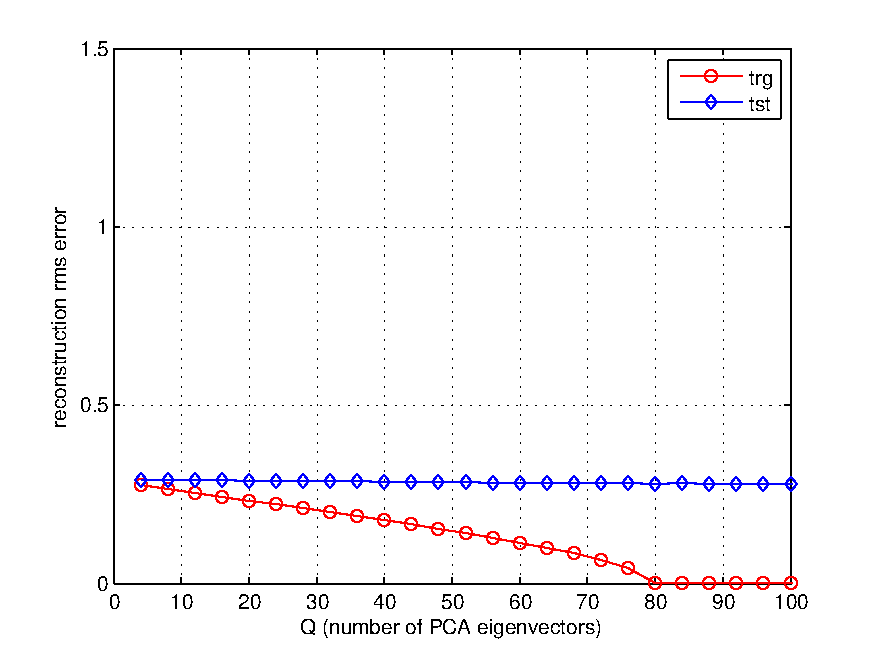
\includegraphics[width=0.3\textwidth]{thesis/PCA_Uniform.pdf}}
\subfigure[Gaussian.]{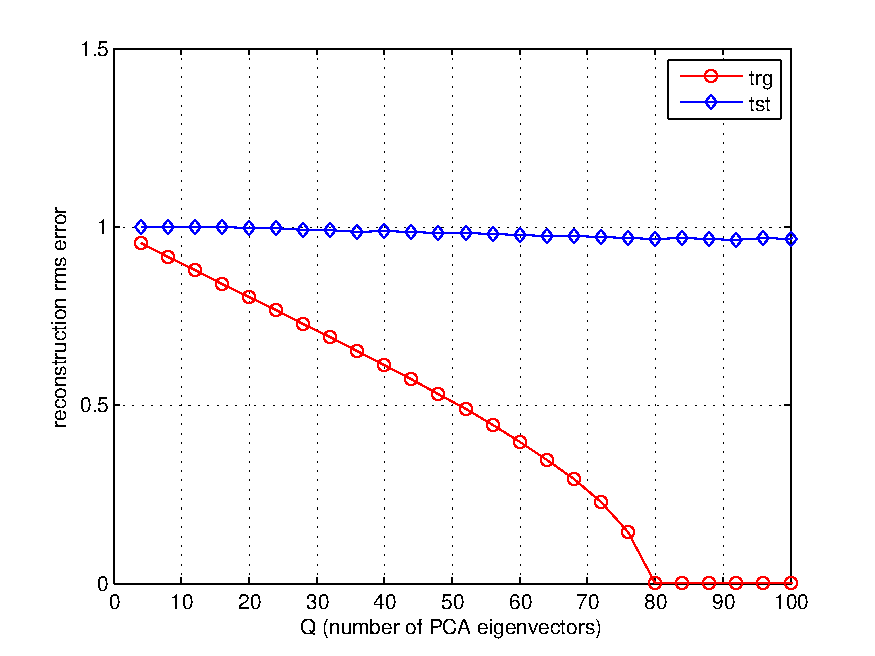
\includegraphics[width=0.3\textwidth]{thesis/PCA_Gaussian.pdf}}
\subfigure[Gauss-Markov.]{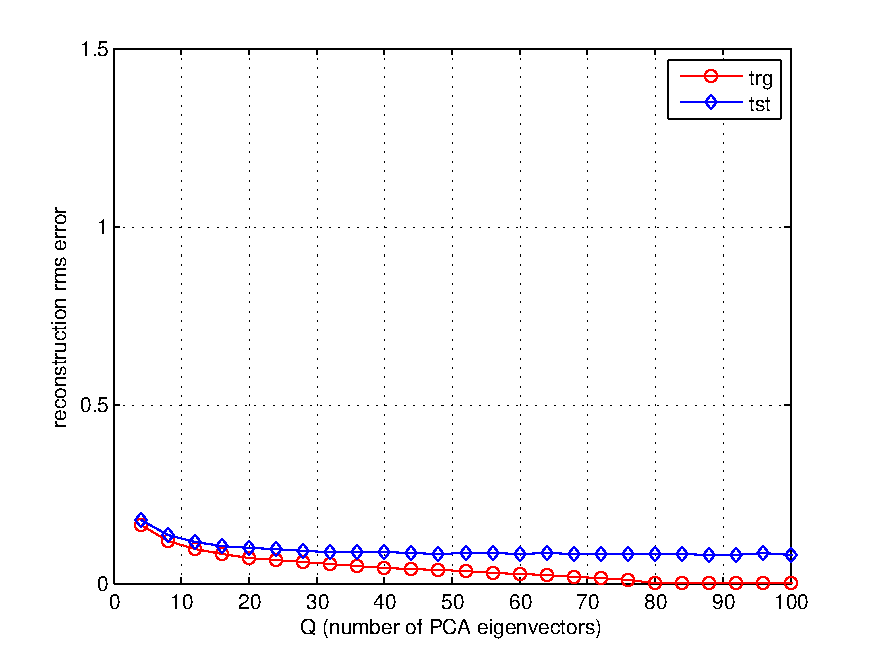
\includegraphics[width=0.3\textwidth]{thesis/PCA_GaussMarkov.pdf}}\hspace{0.55in}
\subfigure[Dudek sequence.]{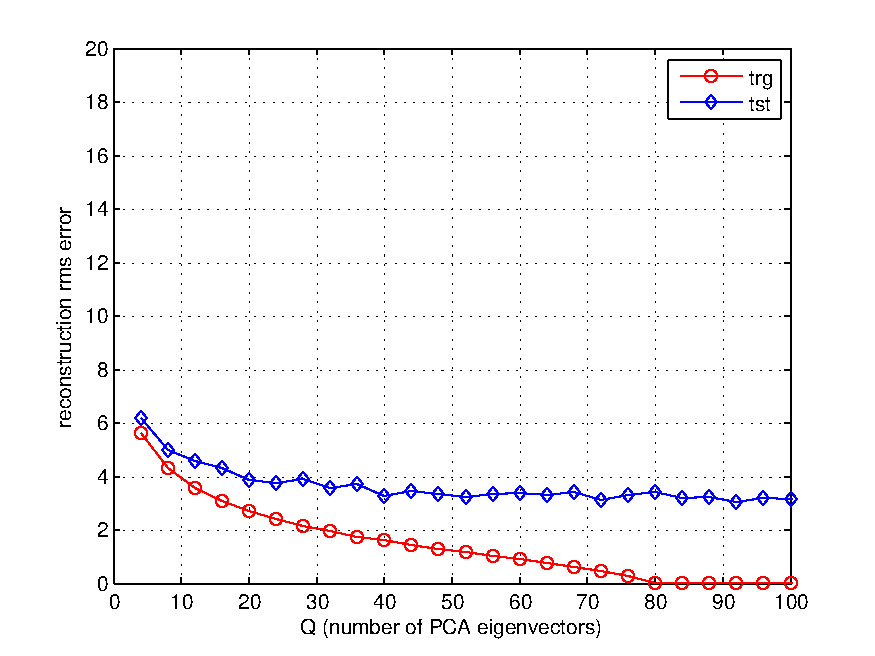
\includegraphics[width=0.3\textwidth]{thesis/PCA_Dudek.pdf}}
\label{fig:PCA_results}
\end{figure}
\end{frame}

%%===================================================
%\subsection{\ \ \ \ usage: video analysis}
%%===================================================
%\begin{frame}
%\frametitle{Action recognition using RVQ}
%\framesubtitle{Weizmann dataset}
%\logoCSIPCPL
%	10 different actions to be classified
%	\begin{figure}	
%		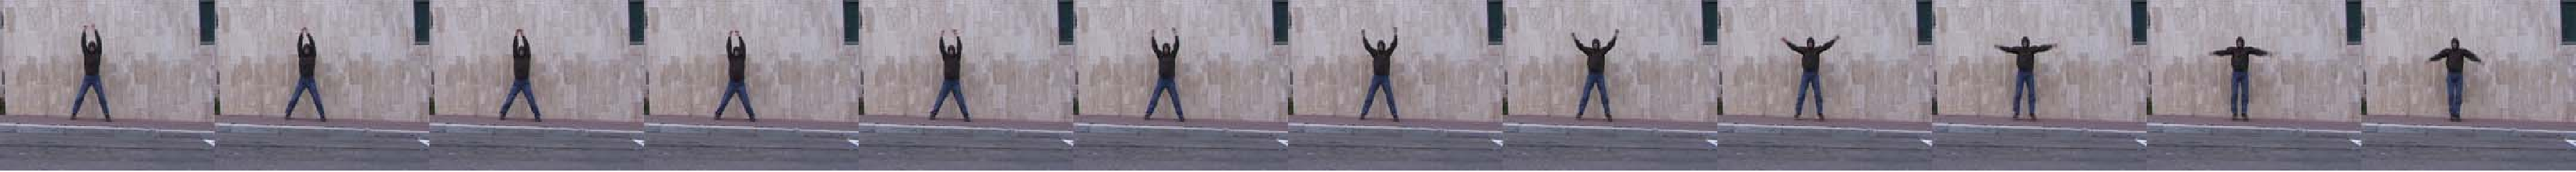
\includegraphics[width=1.0\textwidth]{thesis/RVQ_HMM_IPCV2010_Weizmann_dataset.pdf}
%	\end{figure}
%	\hspace{0.6in}
%	\multiinclude[<+>][format=jpg, start=0, graphics={width=0.6\textwidth}]{thesis/RVQ_HMM_denis_silhouette}
%\end{frame}
%
%
%\begin{frame}[plain]
%\frametitle{Action recognition using RVQ}
%	\begin{changemargin}{-1.3in}{0in}
%	\begin{figure}	
%		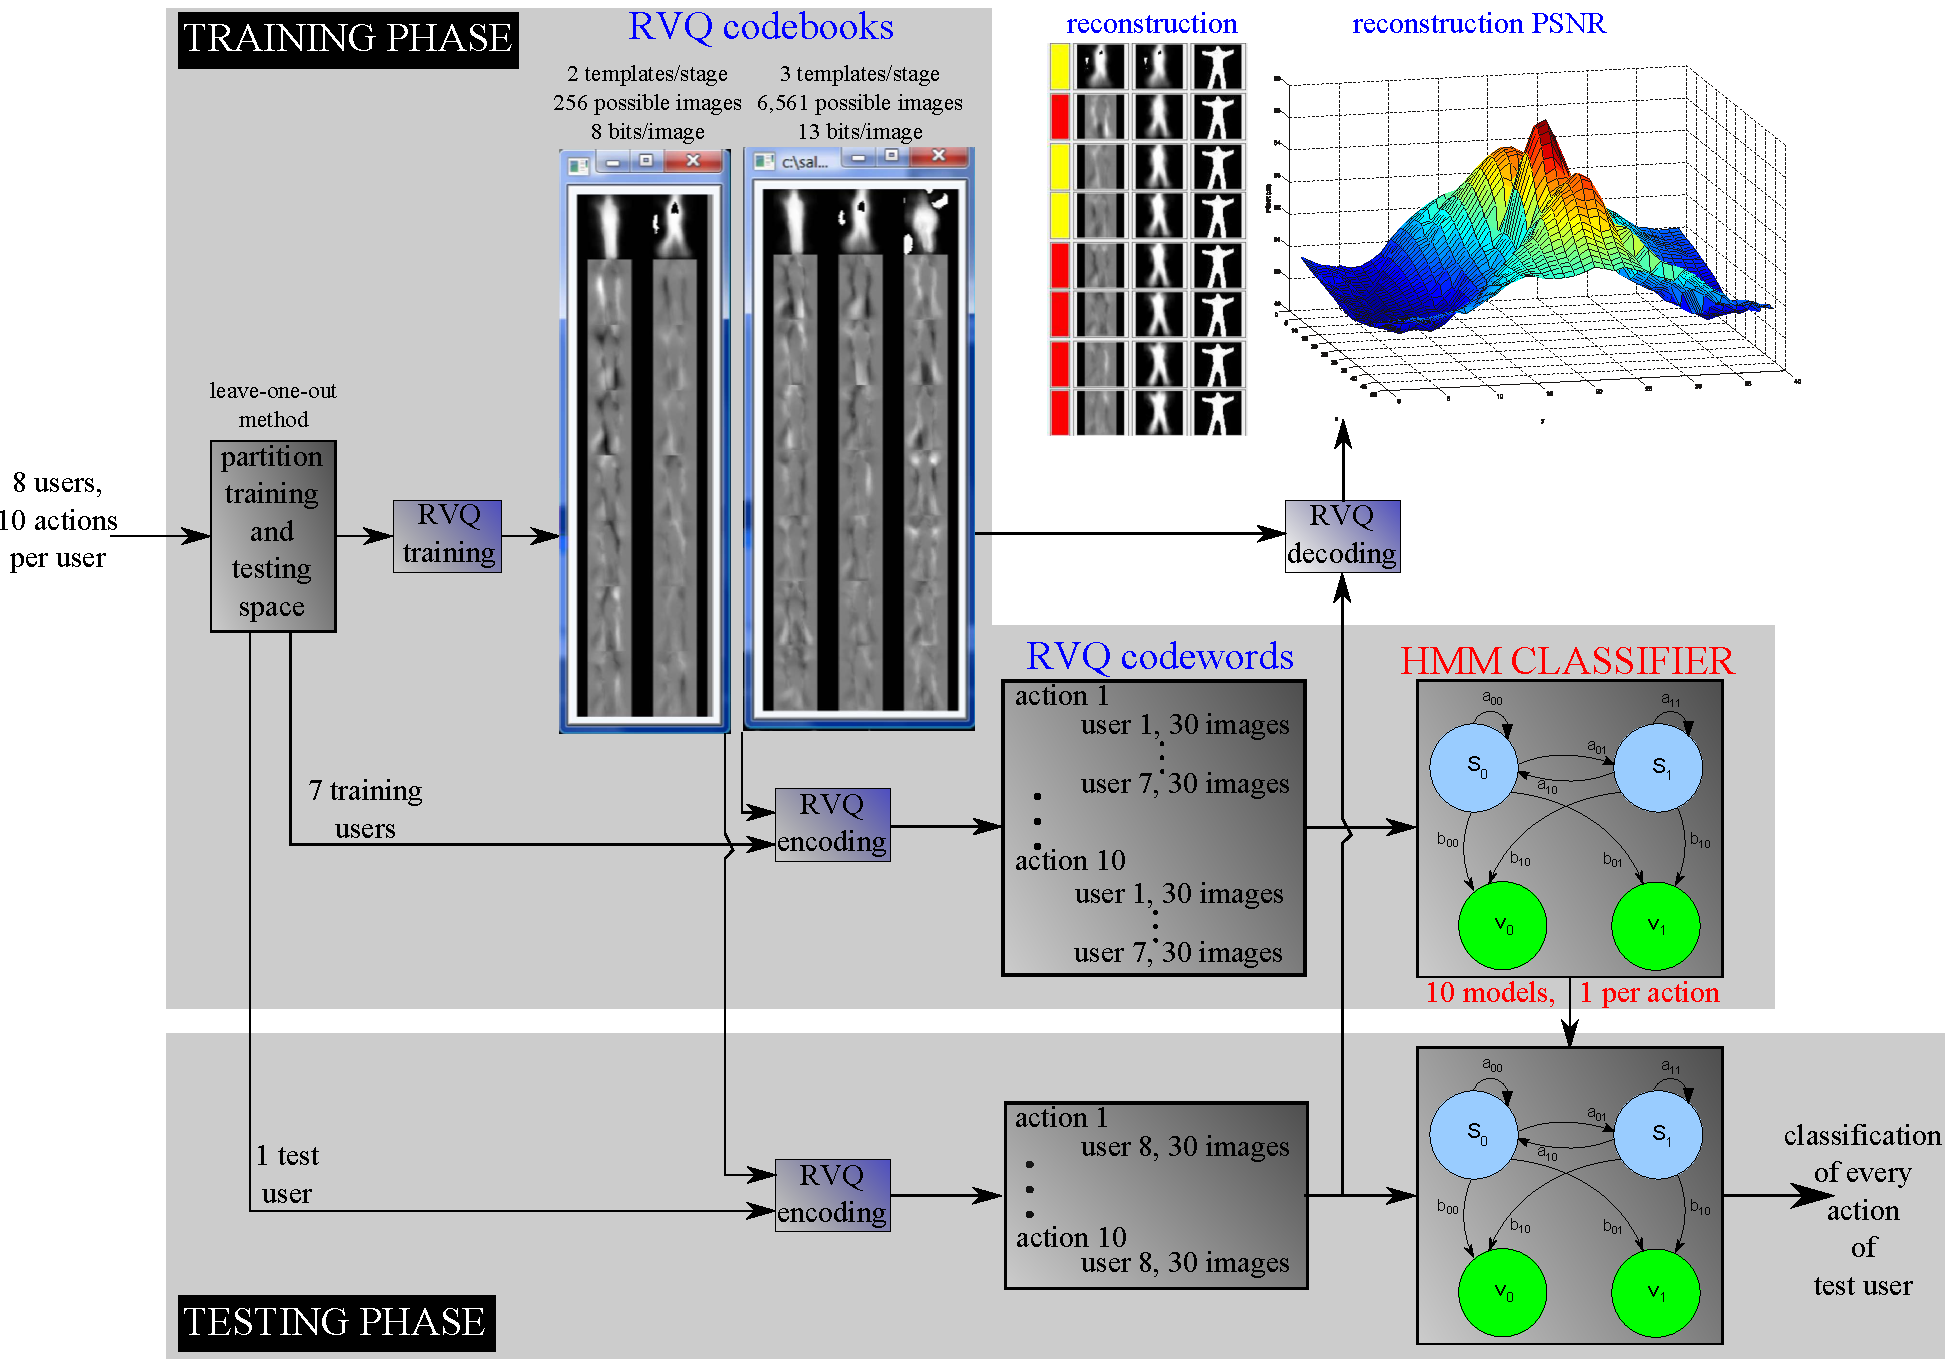
\includegraphics[width=1.35\textwidth]{thesis/RVQ_HMM_IPCV2010_blockDiagram.pdf}
%	\end{figure}
%	\end{changemargin}
%\end{frame}
%
%
%\begin{frame}
%\frametitle{Action recognition using RVQ}
%\framesubtitle{action confusion (all methods: fixed windows)	 \tiny{\footnote{S. M. Aslam, C. F. Barnes, and A. F. Bobick, Video action recognition using residual vector quantization and hidden markov models," in \emph{International Conference on Image Processing, Computer Vision, and Pattern Recognition, 2010}.}}}
%\logoCSIPCPL
%	\begin{figure}
%		\centering	
%		\subfigure[Our method]
%		{
%			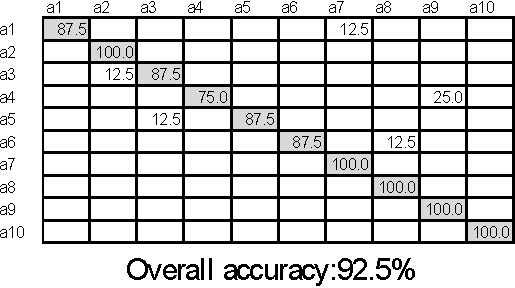
\includegraphics[width=.45\textwidth]{thesis/Proposal_fig7a_RVQ_HMM_Weizmann_TabularResults_us.pdf}
%			\label{fig:Weizmann_TabularResults_us}	
%		}
%		\subfigure[Gorelick et al.]
%		{
%			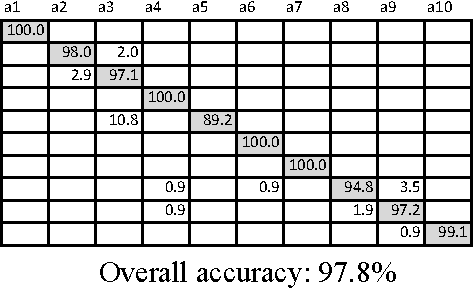
\includegraphics[width=0.40\textwidth]{thesis/Proposal_fig7b_RVQ_HMM_Weizmann_TabularResults_gorelick.pdf}
%			\label{fig:Weizmann_TabularResults_gorelick}	
%		}
%		\subfigure[Manor et al.]
%		{
%			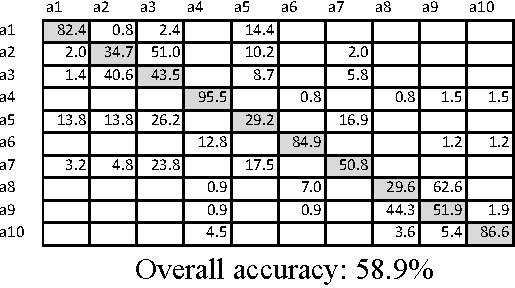
\includegraphics[width=0.45\textwidth]{thesis/Proposal_fig7c_RVQ_HMM_Weizmann_TabularResults_manor.pdf}
%			\label{fig:Weizmann_TabularResults_irani}	
%		}
%		\subfigure[Ali et al.]
%		{
%			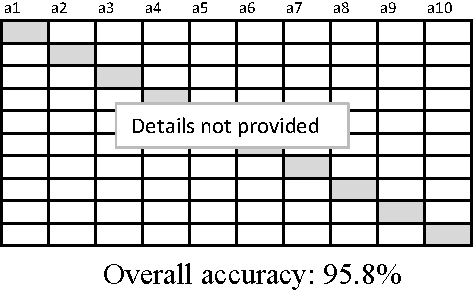
\includegraphics[width=0.40\textwidth]{thesis/Proposal_fig7d_RVQ_HMM_Weizmann_TabularResults_shah.pdf}
%			\label{fig:Weizmann_TabularResults_shah}	
%		}												
%		\label{fig:Weizmann_TabularResults}			
%	\end{figure}
%\end{frame}





\begin{frame}
\frametitle{}
\logoCSIPCPL\mypagenum
		QUESTIONS
\end{frame}

%####################################################################################################
%####################################################################################################
%\bibliographystyle{ieee}
%\bibliography{c:/salman/work/writing/MyCitations}
\end{document}
%####################################################################################################

%####################################################################################################

